\documentclass[12pt, a4paper, spanish]{report}

% Paquetes requeridos
\usepackage[utf8]{inputenc}
\usepackage[spanish]{babel}
\usepackage[margin=1in]{geometry}
\usepackage{graphicx}
\usepackage{booktabs}
\usepackage{array}
\usepackage{fancyhdr}
\usepackage{setspace}
\usepackage{hyperref}
\usepackage{listings}
\usepackage{url}
\usepackage{xcolor}
\usepackage{amsmath,amssymb}
\graphicspath{{figures/}}

% Small adjustment for fancyhdr
\setlength{\headheight}{15pt}

% Minimal Julia language definition for listings (keeps document portable)
\lstdefinelanguage{Julia}{
    morekeywords={function,end,if,else,elseif,while,for,return,struct,module,using,import,begin,let,do,try,catch,finally,break,continue,local,global},
    sensitive=true,
    morecomment=[l]{\#},
    morestring=[b]" ,
    morestring=[b]'
}

% Configuración de listings para código
\lstset{
        language=Julia,
        basicstyle=\ttfamily\small,
        keywordstyle=\color{blue},
        commentstyle=\color{gray},
        stringstyle=\color{red},
        breaklines=true,
        showstringspaces=false,
        frame=single
}

% Espaciado
\onehalfspacing

% Encabezados y pies de página
\pagestyle{fancy}
\fancyhf{}
\fancyhead[R]{\thepage}
\renewcommand{\headrulewidth}{0pt}

\title{}
\author{}
\date{}

\begin{document}

% ============================================================================
% PORTADA
% ============================================================================
\begin{titlepage}
    \centering
    \vspace*{1cm}
    
    {\large \textbf{UNIVERSIDAD DE LA HABANA} \\[0.2cm]
    Facultad de Matemática y Computación \\[0.5cm]}
    
    \vspace{2cm}
    
    {\Large \textbf{Simulación basada en Eventos Discretos} \\[0.3cm]
    \textbf{Poblado en Evolución}}
    
    \vspace{2cm}
    
    {\large Informe}
    
    \vspace{3cm}
    
    {\large
    \texttt{Sebastian González Alfonso} \\[0.5cm]
    \texttt{C312} \\[0.5cm]
    }
    
    \vspace{3cm}
    
    \vfill
    
    {\large \today}
    
\end{titlepage}

% ============================================================================
% ABSTRACT - RESUMEN
% ============================================================================
\addcontentsline{toc}{chapter}{Abstract}

\textbf{Abstract} 

This work presents a concise Julia-based discrete-event simulator for population dynamics that models births, deaths, partnerships and fertility with age-dependent rules. The implementation supports reproducible multi-run experiments with aggregated CSV outputs and standard-error estimates, and includes Python plotting tools for visualization and sensitivity analysis.


\textit{Keywords: discrete event simulation, population dynamics, agent-based model, demographic simulation, Julia, python}

\vspace{1em}

\addcontentsline{toc}{chapter}{Resumen}

\textbf{Resumen}

Se presenta un simulador en Julia de eventos discretos para dinámicas poblacionales (nacimientos, defunciones, formación de parejas y fertilidad) basado en reglas dependientes de la edad. El sistema permite experimentos replicados con exportación de CSV agregados y errores estándar, e incluye herramientas en Python para visualización y análisis de sensibilidad.


\textit{Palabras clave: simulación de eventos discretos, dinámica de poblaciones, modelo basado en agentes, simulación demográfica, Julia, Python}


% ============================================================================
% INTRODUCCIÓN
% ============================================================================
\chapter*{Introducción}
\phantomsection
\addcontentsline{toc}{chapter}{Introducción}

La simulación de sistemas complejos es una herramienta fundamental en la investigación científica y la toma de decisiones. En particular, la simulación de poblaciones humanas permite estudiar cómo factores demográficos y sociales influyen en la evolución temporal de una comunidad.

Este proyecto implementa un simulador de eventos discretos para modelar la evolución de una población en un período de tiempo determinado, considerando factores tales como:

\begin{itemize}
    \item Tasas de mortalidad dependientes de edad y sexo
    \item Probabilidades de embarazo dependientes de la edad de la mujer
    \item Dinámicas de formación y disolución de parejas
    \item Distribuciones del número deseado de hijos
    \item Probabilidades de embarazos múltiples
    \item Períodos de disponibilidad (búsqueda de pareja) con duración estocástica
\end{itemize}

El modelo permite realizar tanto simulaciones individuales como experimentos estadísticos que proporcionan información sobre la sensibilidad de los resultados a variaciones en parámetros demográficos clave. Los resultados se exportan en formato CSV con estadísticas agregadas incluyendo errores estándar.

% ============================================================================
% TABLA DE CONTENIDOS
% ============================================================================
\tableofcontents
\newpage

% ============================================================================
% CAPÍTULO 1: ORDEN DEL PROBLEMA
% ============================================================================
\chapter{Orden del Problema Asignado}

\section{Descripción General}

El problema consiste en simular la evolución de una población en una región determinada durante un período de 100 años. La población inicial está compuesta por $M$ mujeres y $H$ hombres, donde cada individuo tiene una edad inicial distribuida uniformemente en el intervalo $U(0, 100)$.

Se requiere determinar cómo evoluciona la población considerando diversos procesos demográficos regidos por reglas probabilísticas específicas.

\section{Procesos Demográficos}

\subsection{Mortalidad}

La probabilidad de fallecimiento de una persona distribuye uniforme y depende de la edad y el sexo según \ref{table:mortality}.

\begin{table}[h]
    \centering
    \caption{Probabilidad de fallecimiento por grupo de edad y sexo}\label{table:mortality}
    \begin{tabular}{|c|c|c|}
    \hline
    \textbf{Grupo de Edad} & \textbf{Probabilidad Hombres} & \textbf{Probabilidad Mujeres} \\
    \hline
    0--12 & 0.25 & 0.25 \\
    12--45 & 0.10 & 0.15 \\
    45--76 & 0.30 & 0.35 \\
    76--125 & 0.70 & 0.65 \\
    \hline
    \end{tabular}
\end{table}

\subsection{Fertilidad Femenina}

La probabilidad de que una mujer quede embarazada distribuye uniforme y depende de su edad según \ref{table:pregnancy_by_age}. Sin embargo, para que ocurra un embarazo deben satisfacerse las siguientes condiciones:

\begin{itemize}
    \item La mujer debe tener pareja
    \item Ni la mujer ni su pareja deben haber alcanzado su número máximo deseado de hijos
\end{itemize}

\begin{table}[h]
    \centering
    \caption{Probabilidad de embarazo por grupo de edad}\label{table:pregnancy_by_age}
    \begin{tabular}{|c|c|}
    \hline
    \textbf{Grupo de Edad} & \textbf{Probabilidad de Embarazo} \\
    \hline
    12--15 & 0.20 \\
    15--21 & 0.45 \\
    21--35 & 0.80 \\
    35--45 & 0.40 \\
    45--60 & 0.20 \\
    60--125 & 0.05 \\
    \hline
    \end{tabular}
\end{table}

\subsection{Número Deseado de Hijos}

El número de hijos que cada persona desea tener distribuye uniforme según \ref{table:desired_children}.

\begin{table}[h]
    \centering
    \caption{Distribución del número deseado de hijos}\label{table:desired_children}
    \begin{tabular}{|c|c|}
    \hline
    \textbf{Número de Hijos} & \textbf{Probabilidad} \\
    \hline
    1 & 0.60 \\
    2 & 0.75 \\
    3 & 0.35 \\
    4 & 0.20 \\
    5 & 0.10 \\
    5+ & 0.05 \\
    \hline
    \end{tabular}
\end{table}

\subsection{Formación de Parejas}

Para que dos personas formen pareja deben cumplirse las siguientes condiciones:

\begin{enumerate}
    \item Ambas personas deben estar solteras (sin pareja actual)
    \item Ambas personas deben desear tener pareja
    \item Los individuos deben ser de sexo opuesto
\end{enumerate}

La probabilidad de desear pareja depende de la edad según \ref{table:partner_wish}.

\begin{table}[h]
    \centering
    \caption{Probabilidad de desear tener pareja por grupo de edad}
    \begin{tabular}{|c|c|}
    \hline
    \textbf{Grupo de Edad} & \textbf{Probabilidad} \\
    \hline
    12--15 & 0.60 \\
    15--21 & 0.65 \\
    21--35 & 0.80 \\
    35--45 & 0.60 \\
    45--60 & 0.50 \\
    60--125 & 0.20 \\
    \hline
    \end{tabular}
    \label{table:partner_wish}
\end{table}

La probabilidad de que dos personas de diferente sexo que desean pareja se conviertan en pareja depende de la diferencia de edad según \ref{table:partner_by_age_diff}.

\begin{table}[h]
    \centering
    \caption{Probabilidad de establecer pareja por diferencia de edad}\label{table:partner_by_age_diff}
    \begin{tabular}{|c|c|}
    \hline
    \textbf{Diferencia de Edad} & \textbf{Probabilidad} \\
    \hline
    0--5 años & 0.45 \\
    5--10 años & 0.40 \\
    10--15 años & 0.35 \\
    15--20 años & 0.25 \\
    $\geq 20$ años & 0.15 \\
    \hline
    \end{tabular}
\end{table}

\subsection{Ruptura de Parejas}

Cuando dos personas están en pareja, la probabilidad de que ocurra una ruptura es uniforme y constante: $p = 0.2$.

Cuando una persona se separa o enviuda, debe permanecer sola por un período de tiempo que distribuye exponencial con parámetro $\lambda$ dependiente de la edad según \ref{table:isolation_lambda}.

\begin{table}[h]
    \centering
    \caption{Tiempo medio de aislamiento post-separación}\label{table:isolation_lambda}
    \begin{tabular}{|c|c|}
    \hline
    \textbf{Grupo de Edad} & \textbf{Media (meses)} \\
    \hline
    12--15 & 3 \\
    15--21 & 6 \\
    21--35 & 6 \\
    35--45 & 12 \\
    45--60 & 24 \\
    60--125 & 48 \\
    \hline
    \end{tabular}
\end{table}

\subsection{Embarazos Múltiples}

Cuando una mujer queda embarazada, puede tener un embarazo múltiple. El número de bebés distribuye uniforme según \ref{table:multiple_births}.

\begin{table}[h]
    \centering
    \caption{Distribución del número de bebés en un embarazo}\label{table:multiple_births}
    \begin{tabular}{|c|c|}
    \hline
    \textbf{Número de Bebés} & \textbf{Probabilidad} \\
    \hline
    1 & 0.70 \\
    2 & 0.18 \\
    3 & 0.08 \\
    4 & 0.04 \\
    5 & 0.02 \\
    \hline
    \end{tabular}
\end{table}

\subsection{Sexo de Nacidos}

La probabilidad del sexo de cada bebé nacido es uniforme: $P(\text{masculino}) = P(\text{femenino}) = 0.5$.

% ============================================================================
% ============================================================================
% CAPÍTULO: MARCO TEÓRICO
% ============================================================================
\chapter{Marco Teórico}
\label{ch:marco_teorico}

Este capítulo resume definiciones y herramientas extraídas de la bibliografía básica del curso de Simulación impartida en el segundo semestre de tercer año en la carrera Ciencia de la Computación de la Facultad de Matemática y Computación de la Universidad de La Habana \cite{garcia2006}.

\section{Definiciones fundamentales}

\begin{itemize}
    \item \textbf{Sistema}: conjunto de estructuras (entidades, relaciones)
    y procesos relevantes para el dominio del problema. La representación
    del sistema varía según el nivel de abstracción requerido para el estudio.

    \item \textbf{Modelo}: un modelo es un sistema que representa a otro
    sistema; el modelo conceptual define la especificación (estructuras y
    procesos) que después se implementa como modelo computacional.

    \item \textbf{Simulación}: proceso de ejecución, observación y modificación
    de un modelo (computacional) para estudiar la dinámica del sistema real
    bajo condiciones controladas.

    \item \textbf{Sistema dinámico}: sistema en el que el tiempo es una
    dimensión esencial; puede ser estacionario (estructura fija) o
    no-estacionario (estructura dependiente del tiempo).
\end{itemize}

\section{Herramientas y métodos relevantes}

\subsection{Generación de variables aleatorias}

Existen métodos estándar para generar variables aleatorias. En particular, la \emph{transformada inversa} establece que si $U\sim\mathcal{U}(0,1)$ entonces $X=F^{-1}(U)$ tiene distribución $F$. Este método y las distribuciones
comunes (uniforme, exponencial, Poisson) son la base para simular tiempos hasta
eventos (p. ej. tiempos de aislamiento, tiempos hasta muerte) y probabilidades
de ocurrencia (embarazo, formación de pareja) en nuestro simulador. 

A continuación se presentan fórmulas prácticas utilizadas en el proyecto:

\paragraph{Uniforme continua en $[a,b]$.}
Si $U\sim\mathcal{U}(0,1)$, entonces
$$
X = a + (b-a)\,U,
$$
con esperanza $E[X]=\frac{a+b}{2}$ y varianza $\mathrm{Var}(X)=\frac{(b-a)^2}{12}$.

\paragraph{Uniforme discreta en $\{m,\dots,n\}$.}
Una forma práctica de obtener una variable entera uniforme es
$$
X = m + \left\lfloor (n-m+1)\,U \right\rfloor,
$$
donde $\lfloor\cdot\rfloor$ denota la parte entera y $U\sim\mathcal{U}(0,1)$.

\paragraph{Exponencial.}
Para una exponencial con parámetro de tasa $\lambda>0$ (densidad $f(x)=\lambda e^{-\lambda x}$, $x\ge 0$) la transformada inversa da
$$
X = -\frac{1}{\lambda}\ln(U),
$$
que tiene media $E[X]=1/\lambda$ y varianza $\mathrm{Var}(X)=1/\lambda^2$.
Si en cambio la tabla de parámetros usa $\beta$ como parámetro de escala (media), entonces
$$
X = -\beta\ln(U), \qquad E[X]=\beta,\quad \mathrm{Var}(X)=\beta^2.
$$


\subsection{Simulación basada en eventos discretos}

La arquitectura clásica de simulación por eventos discretos sigue la siguiente estructura:
evento, agenda (lista de eventos), avance de reloj, ejecución y programación
de nuevos eventos. Este esquema es la columna vertebral del motor de simulación
empleado en este proyecto: una cola de eventos ordenada por tiempo, procesamiento
del siguiente evento, actualización del estado y registro de estadísticas.

\subsection{Análisis estadístico de la simulación}

Las herramientas básicas de análisis estadístico son la esperanza (media), la
varianza muestral y los estimadores de error estándar. Para estimar incertidumbres se
recomienda el uso de réplicas independientes (Monte Carlo replicado); en el
proyecto se ejecutaron múltiples réplicas por configuración y se calcularon la
media y el error estándar por punto temporal, exportándolos en CSV para trazado
y análisis.

Denotemos por $X_1,\dots,X_n$ las observaciones obtenidas por $n$ réplicas independientes para una cantidad de interés en un instante dado (p. ej. población total a un año $t$).

\paragraph{Estimador de la media (esperanza muestral).}
$$
\bar{X}=\frac{1}{n}\sum_{i=1}^n X_i.
$$

\paragraph{Estimador de la varianza muestral (no sesgado).}
$$
s^2=\frac{1}{n-1}\sum_{i=1}^n (X_i-\bar{X})^2.
$$

\paragraph{Error estándar de la media.}
$$
\mathrm{SE}(\bar{X})=\frac{s}{\sqrt{n}}.
$$

\paragraph{Estimador de proporciones.}
Para proporciones (p. ej. fracción de mujeres en la población) se usa
$$
\hat{p}=\frac{k}{n},\qquad \mathrm{SE}(\hat{p})=\sqrt{\frac{\hat{p}(1-\hat{p})}{n}}.
$$

En las exportaciones CSV se guardaron la media $\bar{X}$ y el error estándar $\mathrm{SE}(\bar{X})$ por cada punto temporal para permitir la representación de bandas $\bar{X}\pm\mathrm{SE}(\bar{X})$ en los gráficos.

% ============================================================================
% CAPÍTULO 3: PRINCIPALES IDEAS PARA LA SOLUCIÓN
% ============================================================================
\chapter{ Descripción de la solución}

\section{Enfoque General}\label{sec:general_approach}

Para resolver este problema se implementó un simulador basado en eventos discretos con arquitectura modular y extensible. Cada individuo en la población es representado como una entidad con atributos propios (edad, sexo, estado civil, etc.), siguiendo una arquitectura basada en agentes para explotar las bondades de la Programación Orientada a Objetos y reducir el número de contadores que pudieran entorpecer la legibilidad y extensibilidad del código. Se diseñó un sistema centralizado que ordena y ejecuta eventos en orden temporal usando una cola de prioridad (\texttt{MinHeap}), y un objeto que recoge las configuraciones seleccionadas (\texttt{SimConfig}) y que permite el uso de semillas aleatorias para reproducibilidad y de un logger para revisar el funcionamento evento a evento. Existe una separación clara entre simulación, experimentos y visualización que permite la modularidad con la que se concibió la implementación.

Para los distintos procesos estocásticos se utilizaron dos tipos de distribuciones utilizando métodos estándar de la transformada inversa descritos en el Capítulo \ref{ch:marco_teorico}:

\begin{itemize}
    \item \textbf{Uniforme}: para probabilidades de eventos (mortalidad, embarazo, formación de parejas)
    \item \textbf{Exponencial}: para tiempos de espera post-separación
\end{itemize}

Para introducir algunos eventos como muertes, separaciones, casamientos e intentos de embarazo, se añadió un evento adicional no descrito en la orden (YearEndEvent) con el objetivo de analizar al inicio de cada año qué personas podrían fallecer o separarse (a las seleccionadas se les asignó un día uniformemente aleatorio en el año para el evento a ocurrir) y distribuir en cada mes un intento de búsqueda de pareja o de embarazo según el estado civil de cada persona. Se prefirió esta vía a hacer un análisis diario de posibles eventos a ocurrir o a hacer una distribución inicial de eventos (e. g. asignarle a una persona el día de su muerte desde que nace) para lograr más similitud con la realidad (e. g. una mujer depende de su ciclo menstrual para quedar embarazada) y no sobrecargar el simulador con períodos extensos de procesamiento.

Se eligió el lenguaje de programación \texttt{Julia} para el simulador por su legibilidad (comparable con la de \texttt{Python}) y su rapidez (comparable con la de \texttt{C}), dado que otras opciones a analizar presentarían un empeoramiento en alguna de estas dos propiedades. Sin embargo, se usó \texttt{Python} para el graficador por las facilidades que presenta el módulo \texttt{Matplotlib} en la representación científica de datos.

\section{Estructura del Simulador}

El simulador se organiza en los siguientes componentes:

\begin{description}
    \item[Configuración (\texttt{SimConfig}):] Define los parámetros iniciales de la simulación (población inicial, duración, etc.)
    \item[Motor de Eventos (\texttt{EventEngine}):] Gestiona los tipos de eventos y la cola de prioridad necesarios en la simulación
    \item[Gestor de Población (\texttt{PopulationManager}):] Mantiene el estado de la población y dirige el análisis estadístico de los resultados obtenidos al finalizar cada año (o período según las opciones seleccionadas), así como la exportación de estos resultados.
    \item[Módulo de Persona (\texttt{PersonModule}):] Presenta enums necesarios y ofrece una interfaz común a los individuos de la población.
    \item[Módulos estocásticos (\texttt{ProbabilityTables} y \texttt{RandomGenerators}):] Encargados de la generación de variables aleatorias y de la gestión de las distribuciones probabilísticas.
    \item[Dirección de la simulación (\texttt{PopulationSimulator}):] Dirige cada simulación individual orquestando el funcionamiento de cada uno de los componentes.
    \item[Graficador de resultados:] Archivo python que usa seaborn en matplotlib para graficar los resultados de los experimentos realizados, con varias opciones de gráficas.
\end{description}

Se implementaron dos tipos de experimentos:

\begin{enumerate}
    \item \textbf{Evolución Simple (\texttt{SimpleEvolutionExperiment})}: ejecuta múltiples simulaciones independientes (con diferentes semillas aleatorias autoincrementadas desde una base) y agrega estadísticas anuales (media y error estándar) para un análisis estadístico sencillo.
    \item \textbf{Comparación de Parámetros (\texttt{ParameterComparisonExperiment})}: varía un parámetro demográfico clave, ejecuta múltiples simulaciones por valor de parámetro, y compara los resultados finales.
\end{enumerate}


\section{Modelo de simulación de eventos discretos}

Un sistema de eventos discretos se caracteriza porque el estado del sistema cambia únicamente en instantes discretos de tiempo y los cambios de estado están asociados a eventos específicos, por lo que entre ellos el estado permanece constante.

En nuestro modelo, los eventos discretos son:

\begin{itemize}
    \item \textbf{Nacimiento}: una mujer da a luz a uno o más hijos
    \item \textbf{Muerte}: una persona fallece
    \item \textbf{Formación de Pareja}: dos individuos solteros se convierten en pareja
    \item \textbf{Intento de embarazo}: una pareja intenta tener un hijo.
    \item \textbf{Ruptura de pareja}: una pareja se disuelve
    \item \textbf{Fin de espera}: una persona que estaba divorciada o viuda puede buscar pareja nuevamente
    \item \textbf{Búsqueda de pareja}: una persona que está soltera busca una pareja
    \item \textbf{Fin de año}: un año se acaba, se calculan estadísticas y se planifican algunos eventos.
\end{itemize}

El estado de la simulación en cualquier instante $t$ se define por la colección de todos los individuos activos y sus atributos (e. g. edad, sexo, estado civil, número actual y deseado de hijos).

Las transiciones de estado ocurren cuando se ejecutan eventos. Para cada evento se evalúan las condiciones requeridas y se modifican los atributos relevantes del individuo o individuos involucrados. Al terminar estas acciones, añade de ser requerido y posible (según la distribución de probabilidad pertinente) otros eventos a la cola.

En \texttt{PopulationManager} se llevan las variables contadoras necesarias para el análisis estadístico posterior (e. g. muertes, nacimientos, emparejamientos, separaciones).

El algoritmo de simulación sigue el esquema estándar de eventos discretos:

\begin{enumerate}
    \item Inicializar población
    \item Mientras tiempo de simulación $\leq$ duración total, cola de eventos no vacía y población no extinta:
    \begin{enumerate}
        \item Obtener el próximo evento de la cola
        \item Avanzar reloj a tiempo del evento
        \item Ejecutar evento
        \item Actualizar estado del sistema
        \item Registrar estadísticas
    \end{enumerate}
    \item Exportar resultados
\end{enumerate}

Los eventos se generan de acuerdo a los mecanismos descritos en la orden del proyecto, teniendo en cuenta las consideraciones explicadas en la Sección \ref{sec:general_approach}

\section{Colección de Estadísticas}

La simulación recolecta las siguientes estadísticas en intervalos de tiempo discretos (años o períodos definidos):

\begin{itemize}
    \item Población total
    \item Proporción de sexos
    \item Edad promedio
    \item Nacimientos
    \item Muertes
    \item Emparejamientos
    \item Separaciones
    \item Distribución de edades por sexo
\end{itemize}

% ============================================================================
% CAPÍTULO 4: CONSIDERACIONES Y RESULTADOS
% ============================================================================
\chapter{Resultados}

\section{Experimento 1: Evolución Simple}\label{sec:exp1}

\subsection{Objetivo}

Estudiar cómo evoluciona la población en el tiempo bajo los parámetros demográficos especificados.

\subsection{Parámetros Iniciales}

\begin{itemize}
	\item Población inicial: \texttt{2000}
	\item Duración de simulación: \texttt{100}
	\item Número de réplicas por experimento: \texttt{500}
	\item Edad mínima de fertilidad: \texttt{12}
	\item Edad máxima de fertilidad: \texttt{70}
	\item Edad mínima de emparejamiento: \texttt{12}
	\item Edad máxima: \texttt{125}
	\item Semilla: \texttt{16}
\end{itemize}

\subsection{Resultados}

\subsubsection{Dinámica de Población}

Los datos revelan una clara tendencia a la extinción, con una disminución casi exponencial de la población de ambos sexos como puede verse en la Figura \ref{fig:pop_evolution}. En las 500 simulaciones realizadas, la extinción de la población llegó antes del año 70. Esto puede indicar una inconsistencia entre los valores utilizados en la tabla de probabilidad y el sistema utilizado para la simulación. Lo cierto es que la tasa de muertes es mucho más alta que la de natalidad (que depende de disponibilidad de parejas fértiles y de salud de la madre en el tiempo de gestación), lo que impide que la población se regenere correctamente. Debe tenerse en cuenta que el hecho de que se inicialicen las personas con edades que distribuyen uniformemente en $[0, 100]$ deja aproximadamente la mitad de la población en rangos de edades donde es difícil o imposible reproducirse.

\begin{figure}[h]
    \centering
    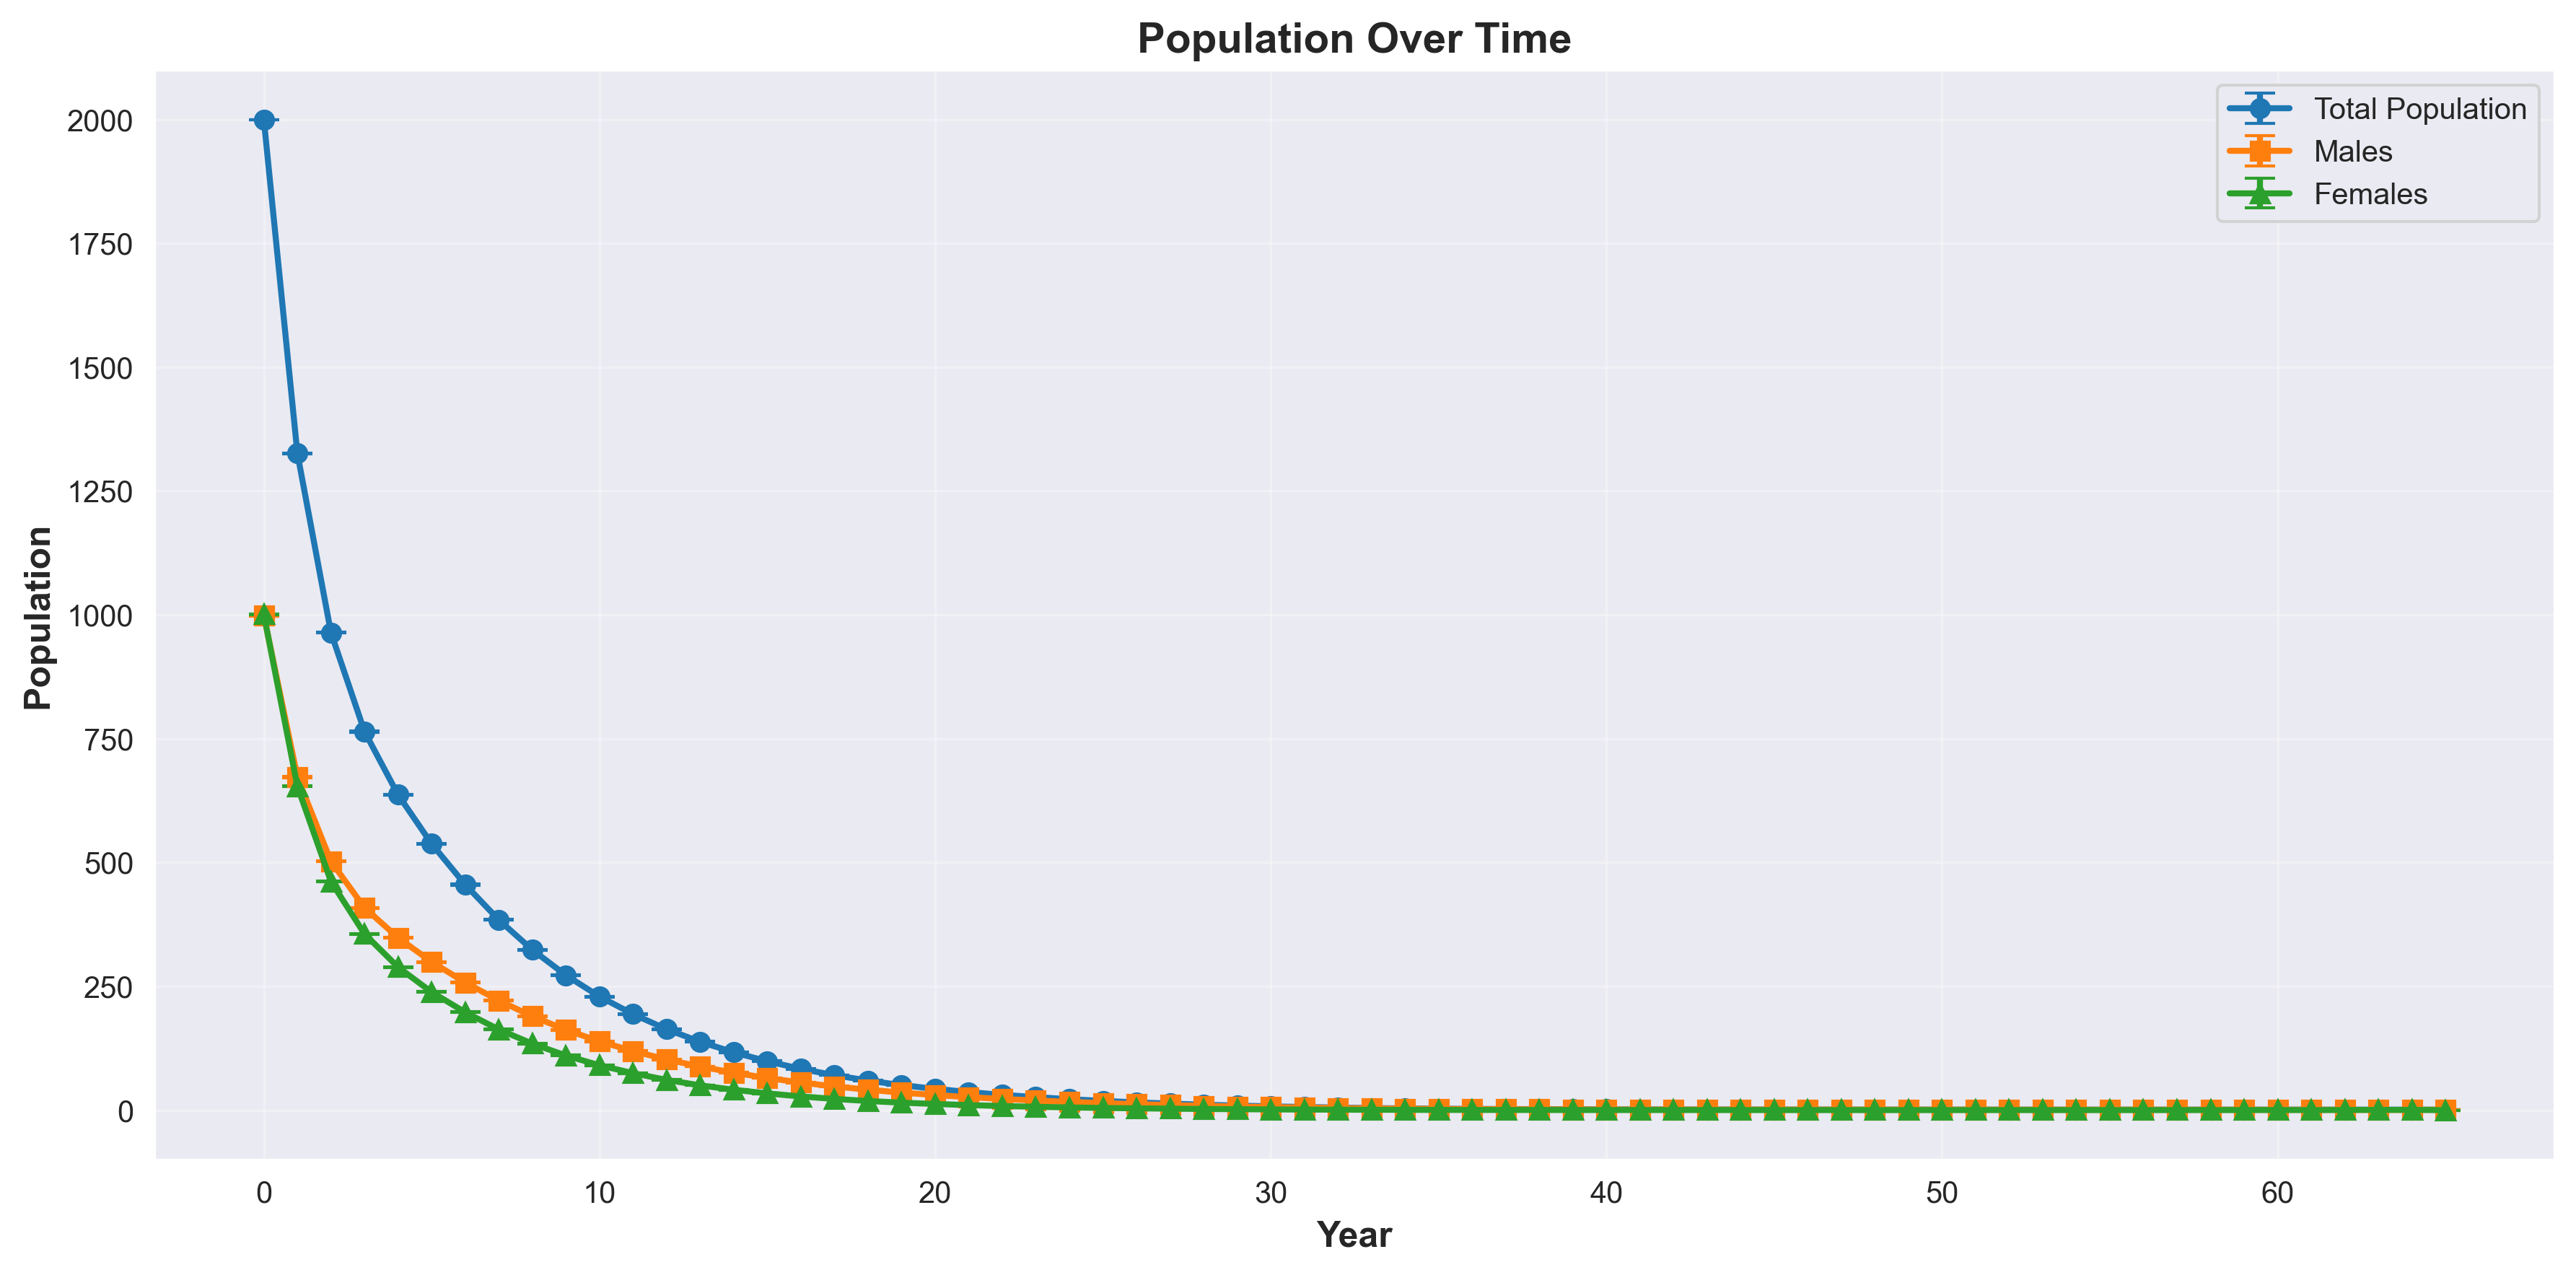
\includegraphics[width=0.9\textwidth]{simple_population_2000.png}
    \caption{Evolución de la población por sexo. Se muestran hombres (naranja), mujeres (verde) y población total (azul). Puede apreciarse la clara tendencia a la extinción, que llega antes del año 70 en todas las simulaciones realizadas.}
    \label{fig:pop_evolution}
\end{figure}


\subsubsection{Dinámicas de Sexos}

El comportamiento de la distribución de sexos en la población es cuanto menos curioso. En los primeros años puede apreciarse una tendencia a la supervivencia de los hombres sobre las mujeres (valores elevados de $M/F$), mientras que hacia el final de la simulación esta tendencia se invierte ligeramente (al acercarse la extinción, las más mínimas diferencias en los números de hombres y mujeres hacen variar significativamente este valor); lo cual puede revisarse en la Figura \ref{fig:sex_ratio}. En general, y como es de esperar al revisar las tablas de probabilidad de mortalidad, los hombres en conjunto son más propensos a sobrevivir que las mujeres. Al revisar los datos, puede verse que los últimos supervivientes de las simulaciones fueron indistintamente hombre o mujer (que se convirtieron en leyendas viviendo solos por 12 años en sus respectivas simulaciones). La explicación de que al final de la simulación el valor de la proporción de sexos caiga a 0 rápidamente es que, al ser una razón, se tomó la decisión de diseño de hacerlo 0 al no quedar ninguna persona de algún sexo (i. e. \texttt{sex\_ratio = 0.0} si \texttt{male\_count = 0} o \texttt{female\_count = 0}).

\begin{figure}[h]
    \centering
    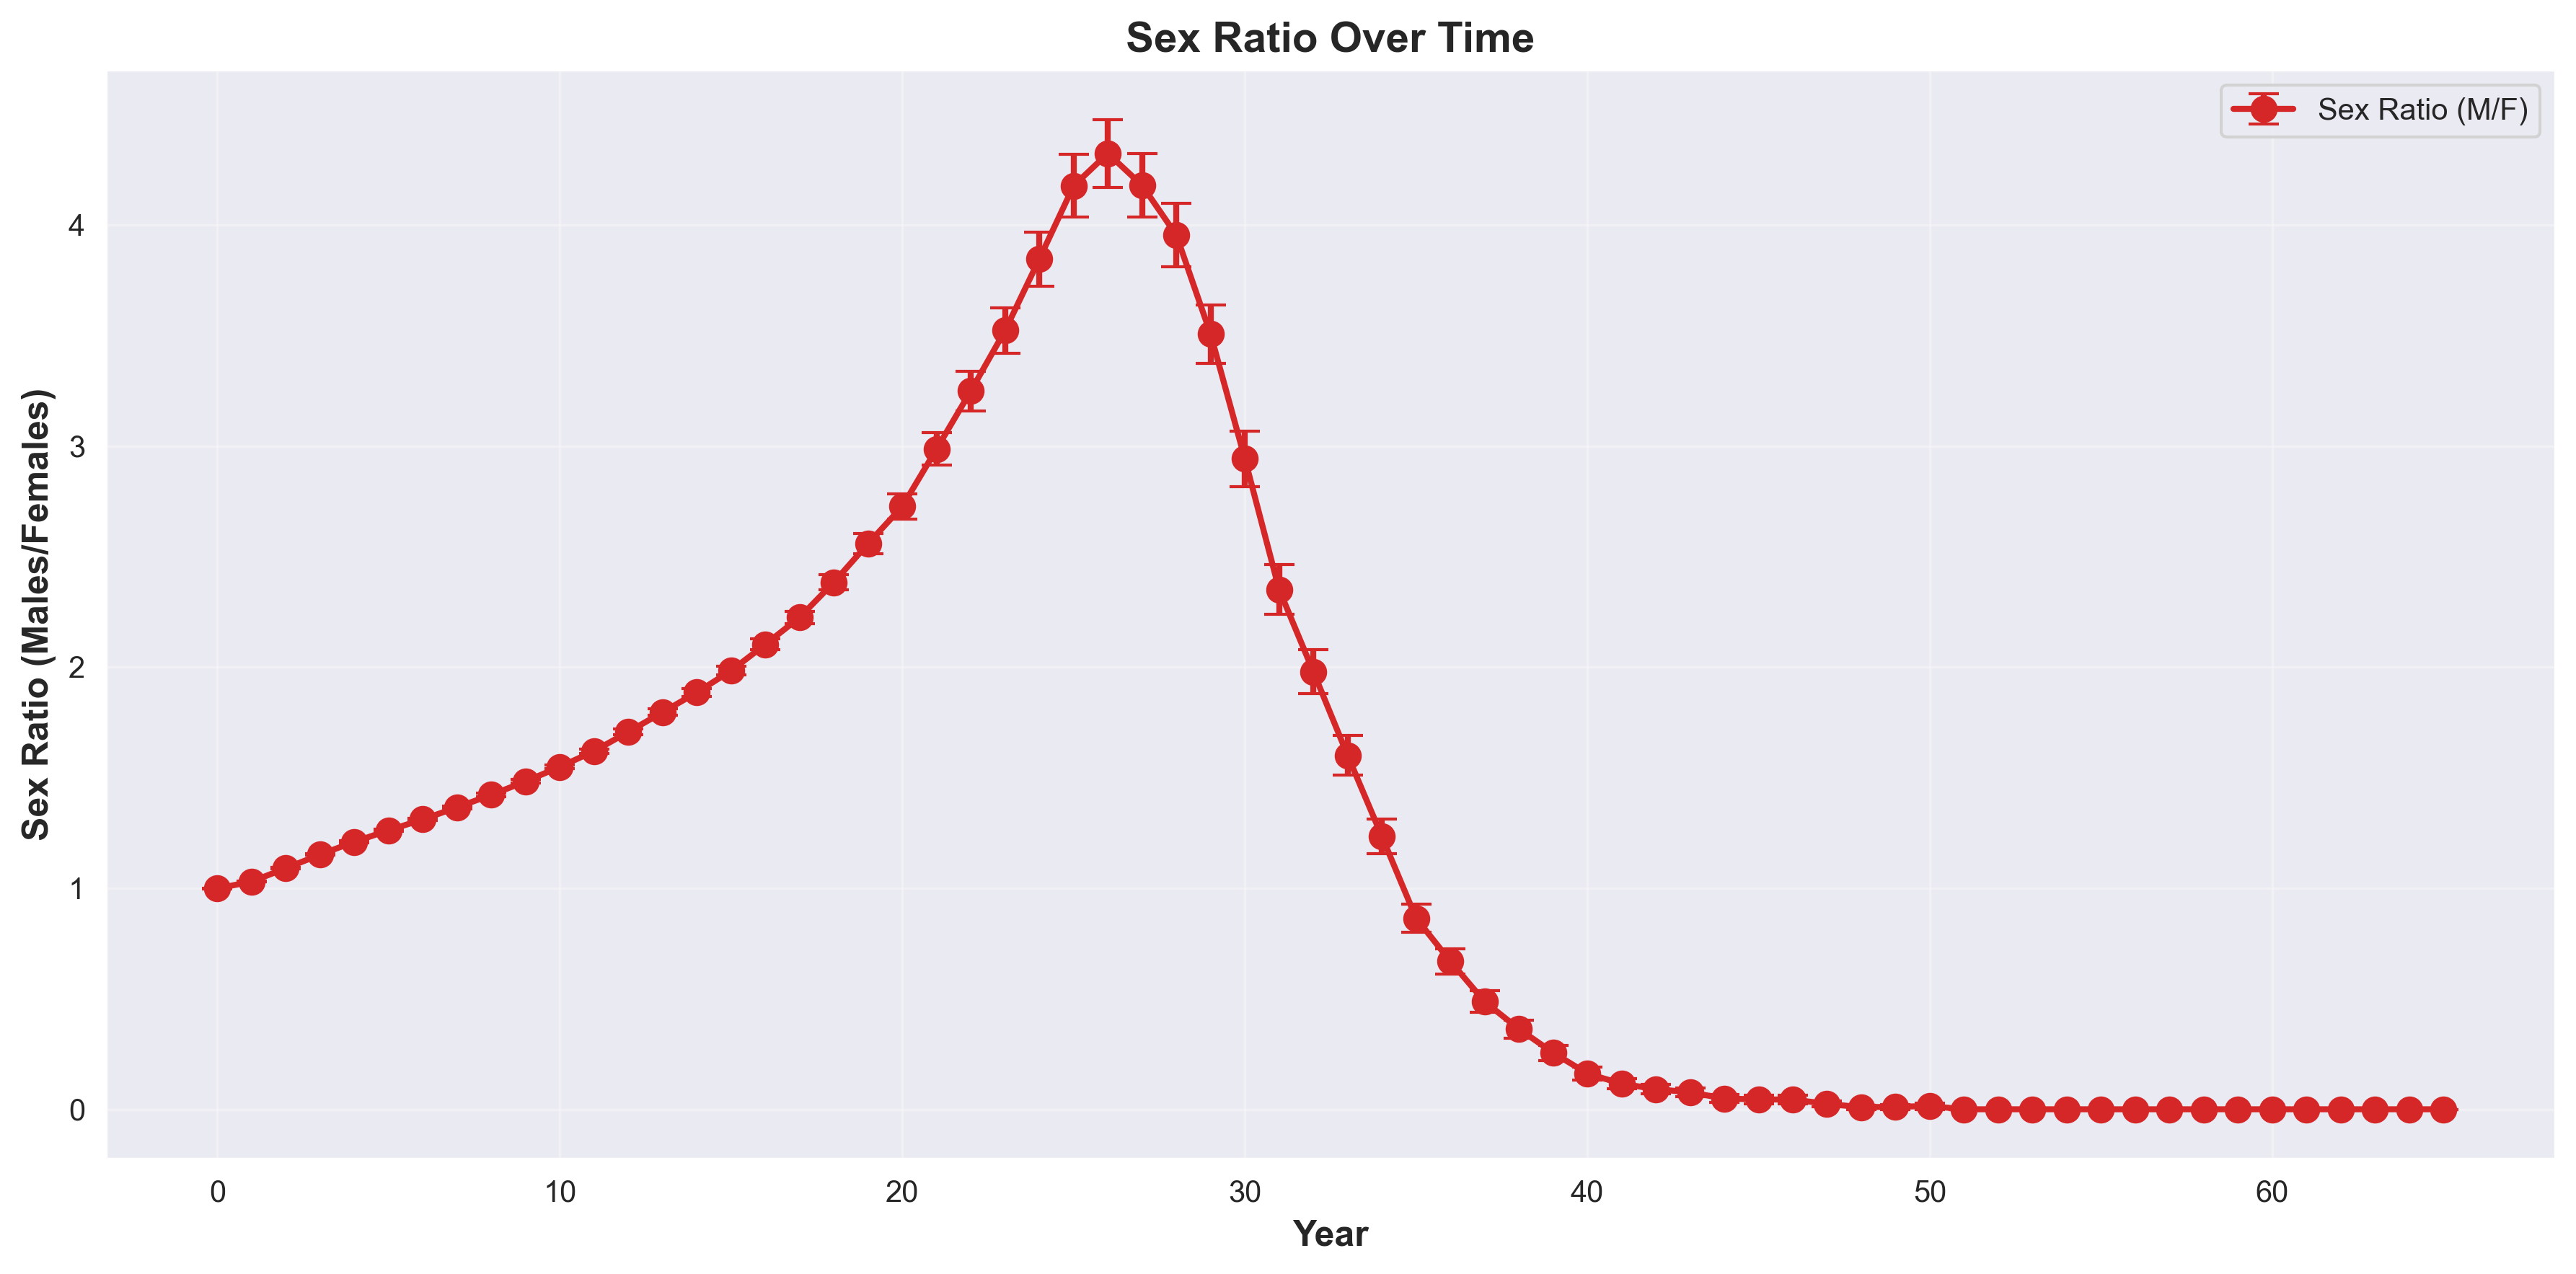
\includegraphics[width=0.9\textwidth]{simple_sratio_2000.png}
    \caption{Razón de sexos (M/F) en función del tiempo de las simulaciones.}
    \label{fig:sex_ratio}
\end{figure}

\subsubsection{Edad Promedio}

La edad promedio muestra un comportamiento predecible en la Figura \ref{fig:avg_age}. Al aumentar con la edad la probabilidad de fallecer, es normal que en los primeros años fallezcan las personas más viejas y se propicie una estabilización de la media de las edades alrededor de 30 años antes de llegar al 10mo año de simulación. Sin embargo, al seguir avanzando el tiempo las personas empiezan a envejecer, lo que, unido con la baja tasa de natalidad presentada, hace que la media de edades vuelva a crecer. A medida que disminuye el número de personas vivas puede presenciarse el ruido estadístico introducido, hasta que queda el último superviviente y solo se grafica su edad.

\begin{figure}[h]
    \centering
    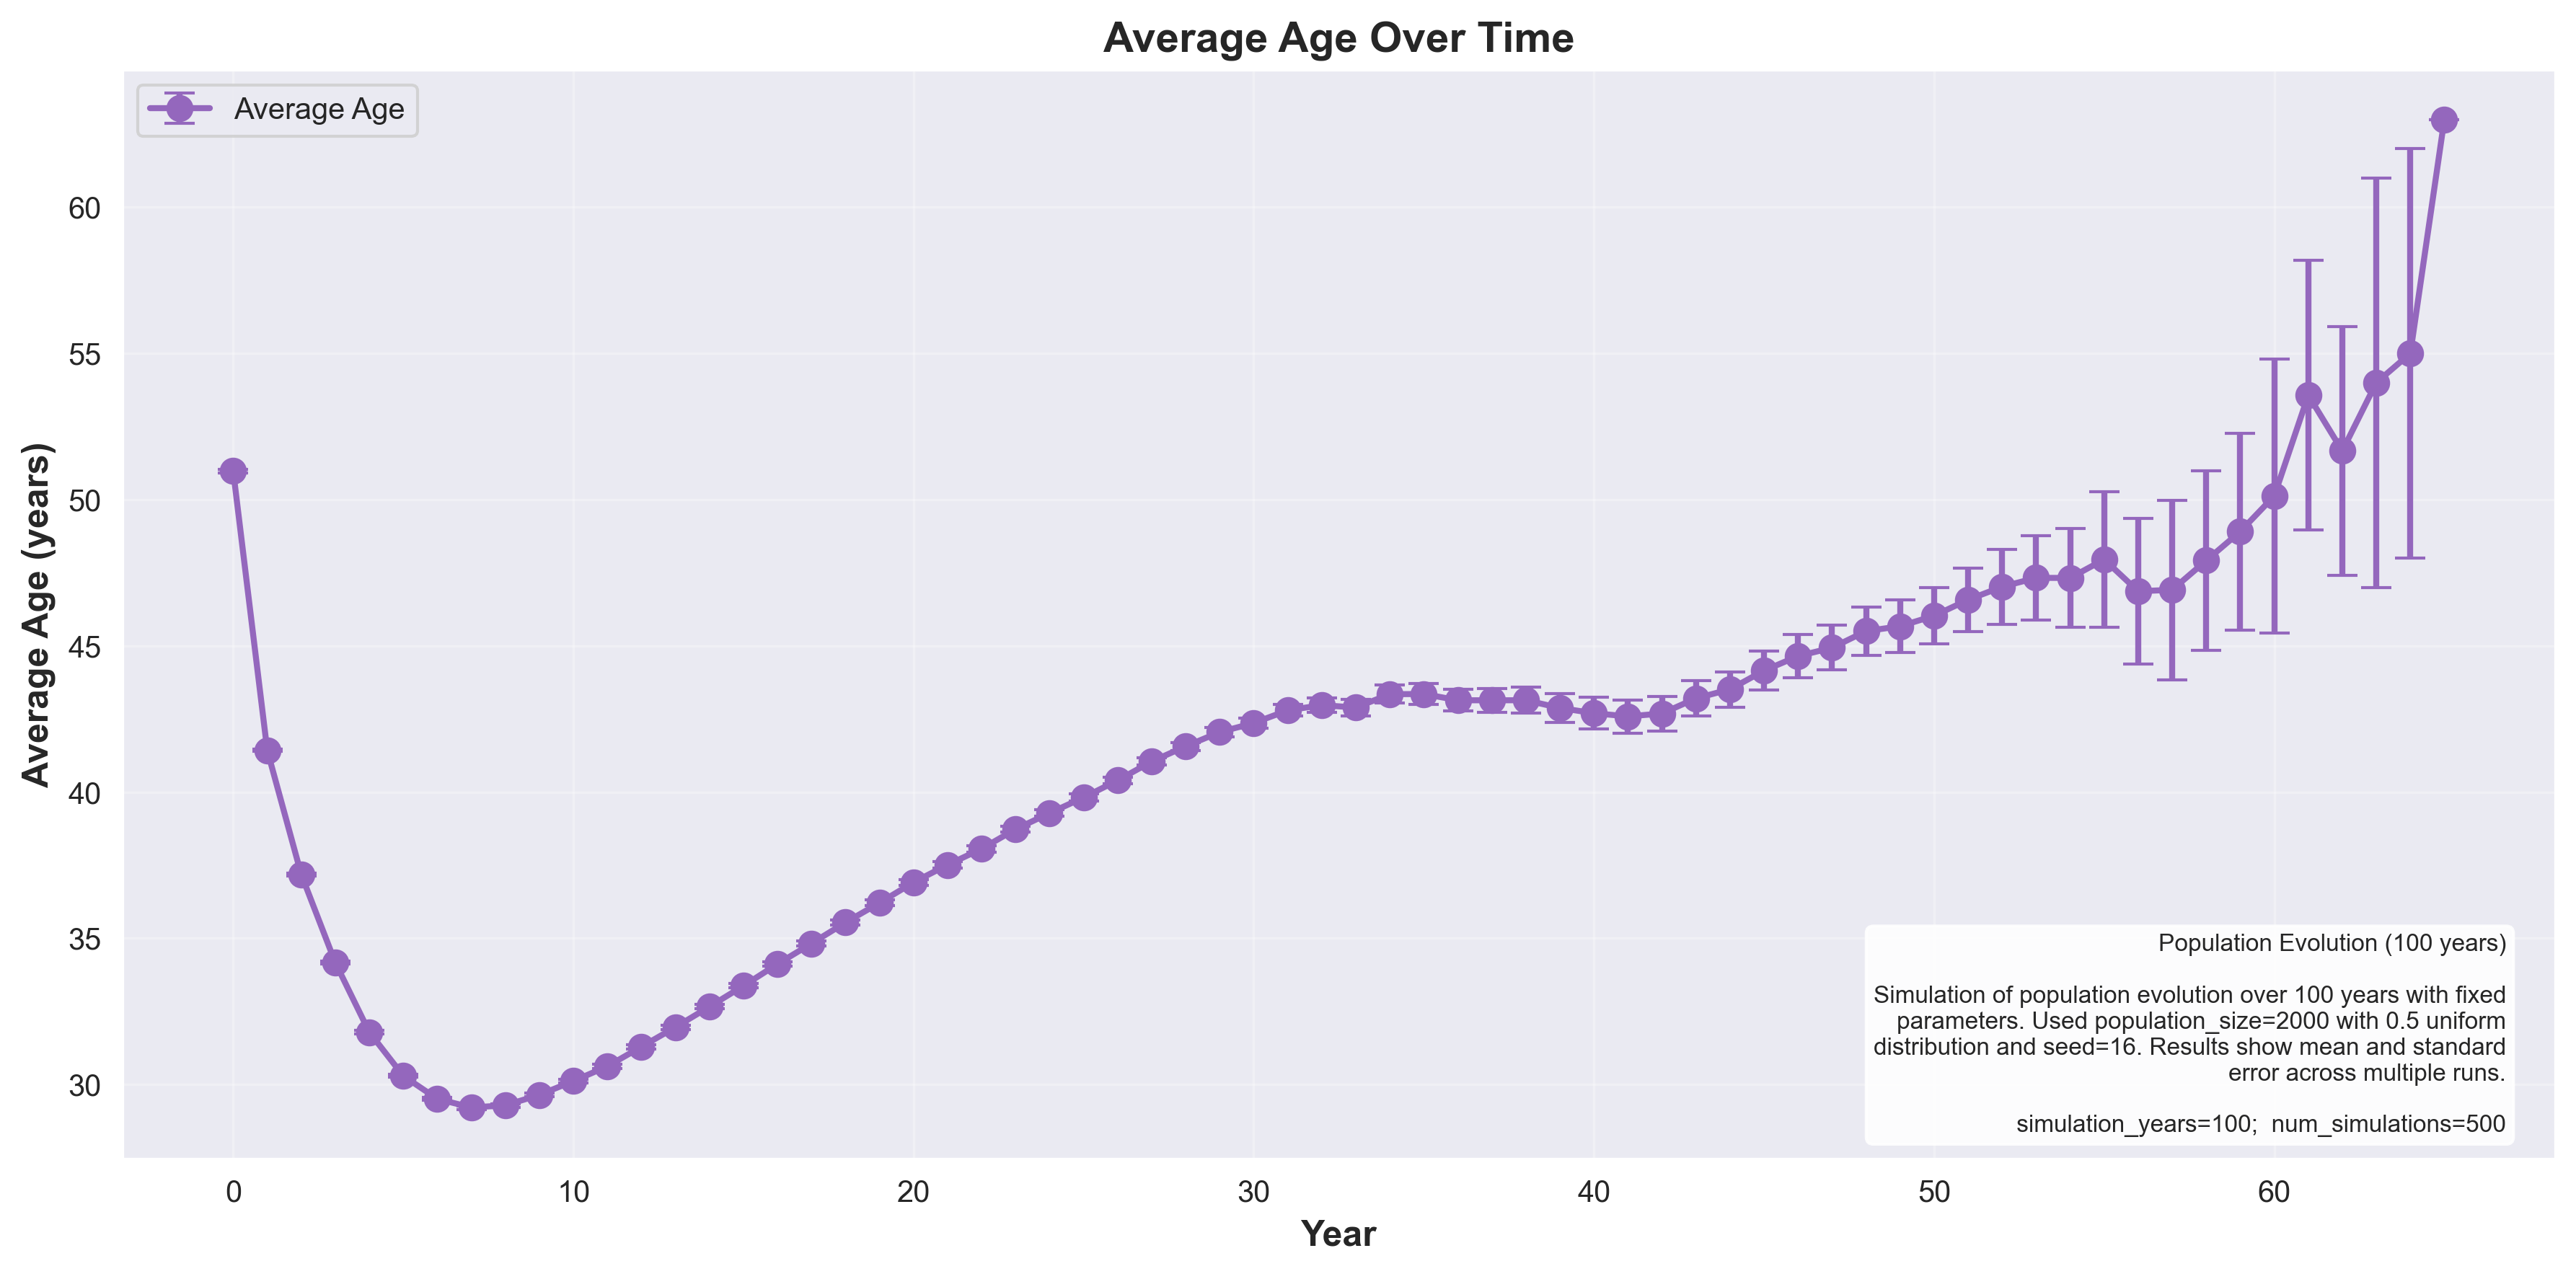
\includegraphics[width=0.9\textwidth]{simple_age_2000.png}
    \caption{Edad promedio de la población en función del tiempo.}
    \label{fig:avg_age}
\end{figure}

\section{Experimento 2: Análisis de Sensibilidad Paramétrica}\label{sec:exp2}

\subsection{Objetivo}

Evaluar cómo cambios en la proporción inicial de hombres en la población afectan la dinámica y la supervivencia poblacional a largo plazo.

\subsection{Parámetros Iniciales}

\begin{itemize}
	\item Población inicial: \texttt{2000}
	\item Población inicial masculina (variado): \texttt{[0, 200, 400, 600, 800, 1000, 1200, 1400, 1600, 1800, 2000]}
	\item Duración de simulación: \texttt{30}
	\item Número de réplicas por parámetro: \texttt{250}
	\item Edad mínima de fertilidad: \texttt{12}
	\item Edad máxima de fertilidad: \texttt{70}
	\item Edad mínima de emparejamiento: \texttt{12}
	\item Edad máxima: \texttt{125}
	\item Semilla base: \texttt{16}
\end{itemize}

Se varió la población inicial masculina desde \texttt{0} (población completamente femenina) hasta \texttt{2000} (población completamente masculina) en intervalos de \texttt{200} individuos. Para cada valor del parámetro se ejecutaron \texttt{250} simulaciones independientes con semillas aleatorias distintas, permitiendo así estimar la media y el error estándar de los resultados para un análisis estadístico robusto.

\subsection{Resultados}

\subsubsection{Dinámica Poblacional}

 El análisis de la Figura \ref{fig:param_pop} revela una situación un tanto curiosa y que puede ser de cierta forma esperada desde el conocimiento de las tablas de probabilidad de mortalidad, claramente desbalanceadas hacia la mujer (i. e. las mujeres tienen generalmente mayor probabilidad de fallecer). La población pasados 30 años era de 2 personas aproximadamente cuando todas eran mujeres (menor valor obtenido), mientras que era de 10 personas aproximadamente cuando todos eran hombres (mayor valor obtenido). Este valor no debe engañarnos y hacernos pensar que una població de solo hombres es más propensa a sobrevivir, pues al pasar el tiempo y no poder recuperarse la producción con nacimientos de nuevos pobladores, la extinción es casi segura. El valor ideal para la población masculina podría fijarse entre 200 y 400, ya que entre estos valores se puede apreciar un mayor equilibrio entre los pobladores de ambos sexos, lo que lo hace prometedor a largo plazo (a pesar de encontrarse ya prácticamente extinta la población).

\begin{figure}[h]
    \centering
    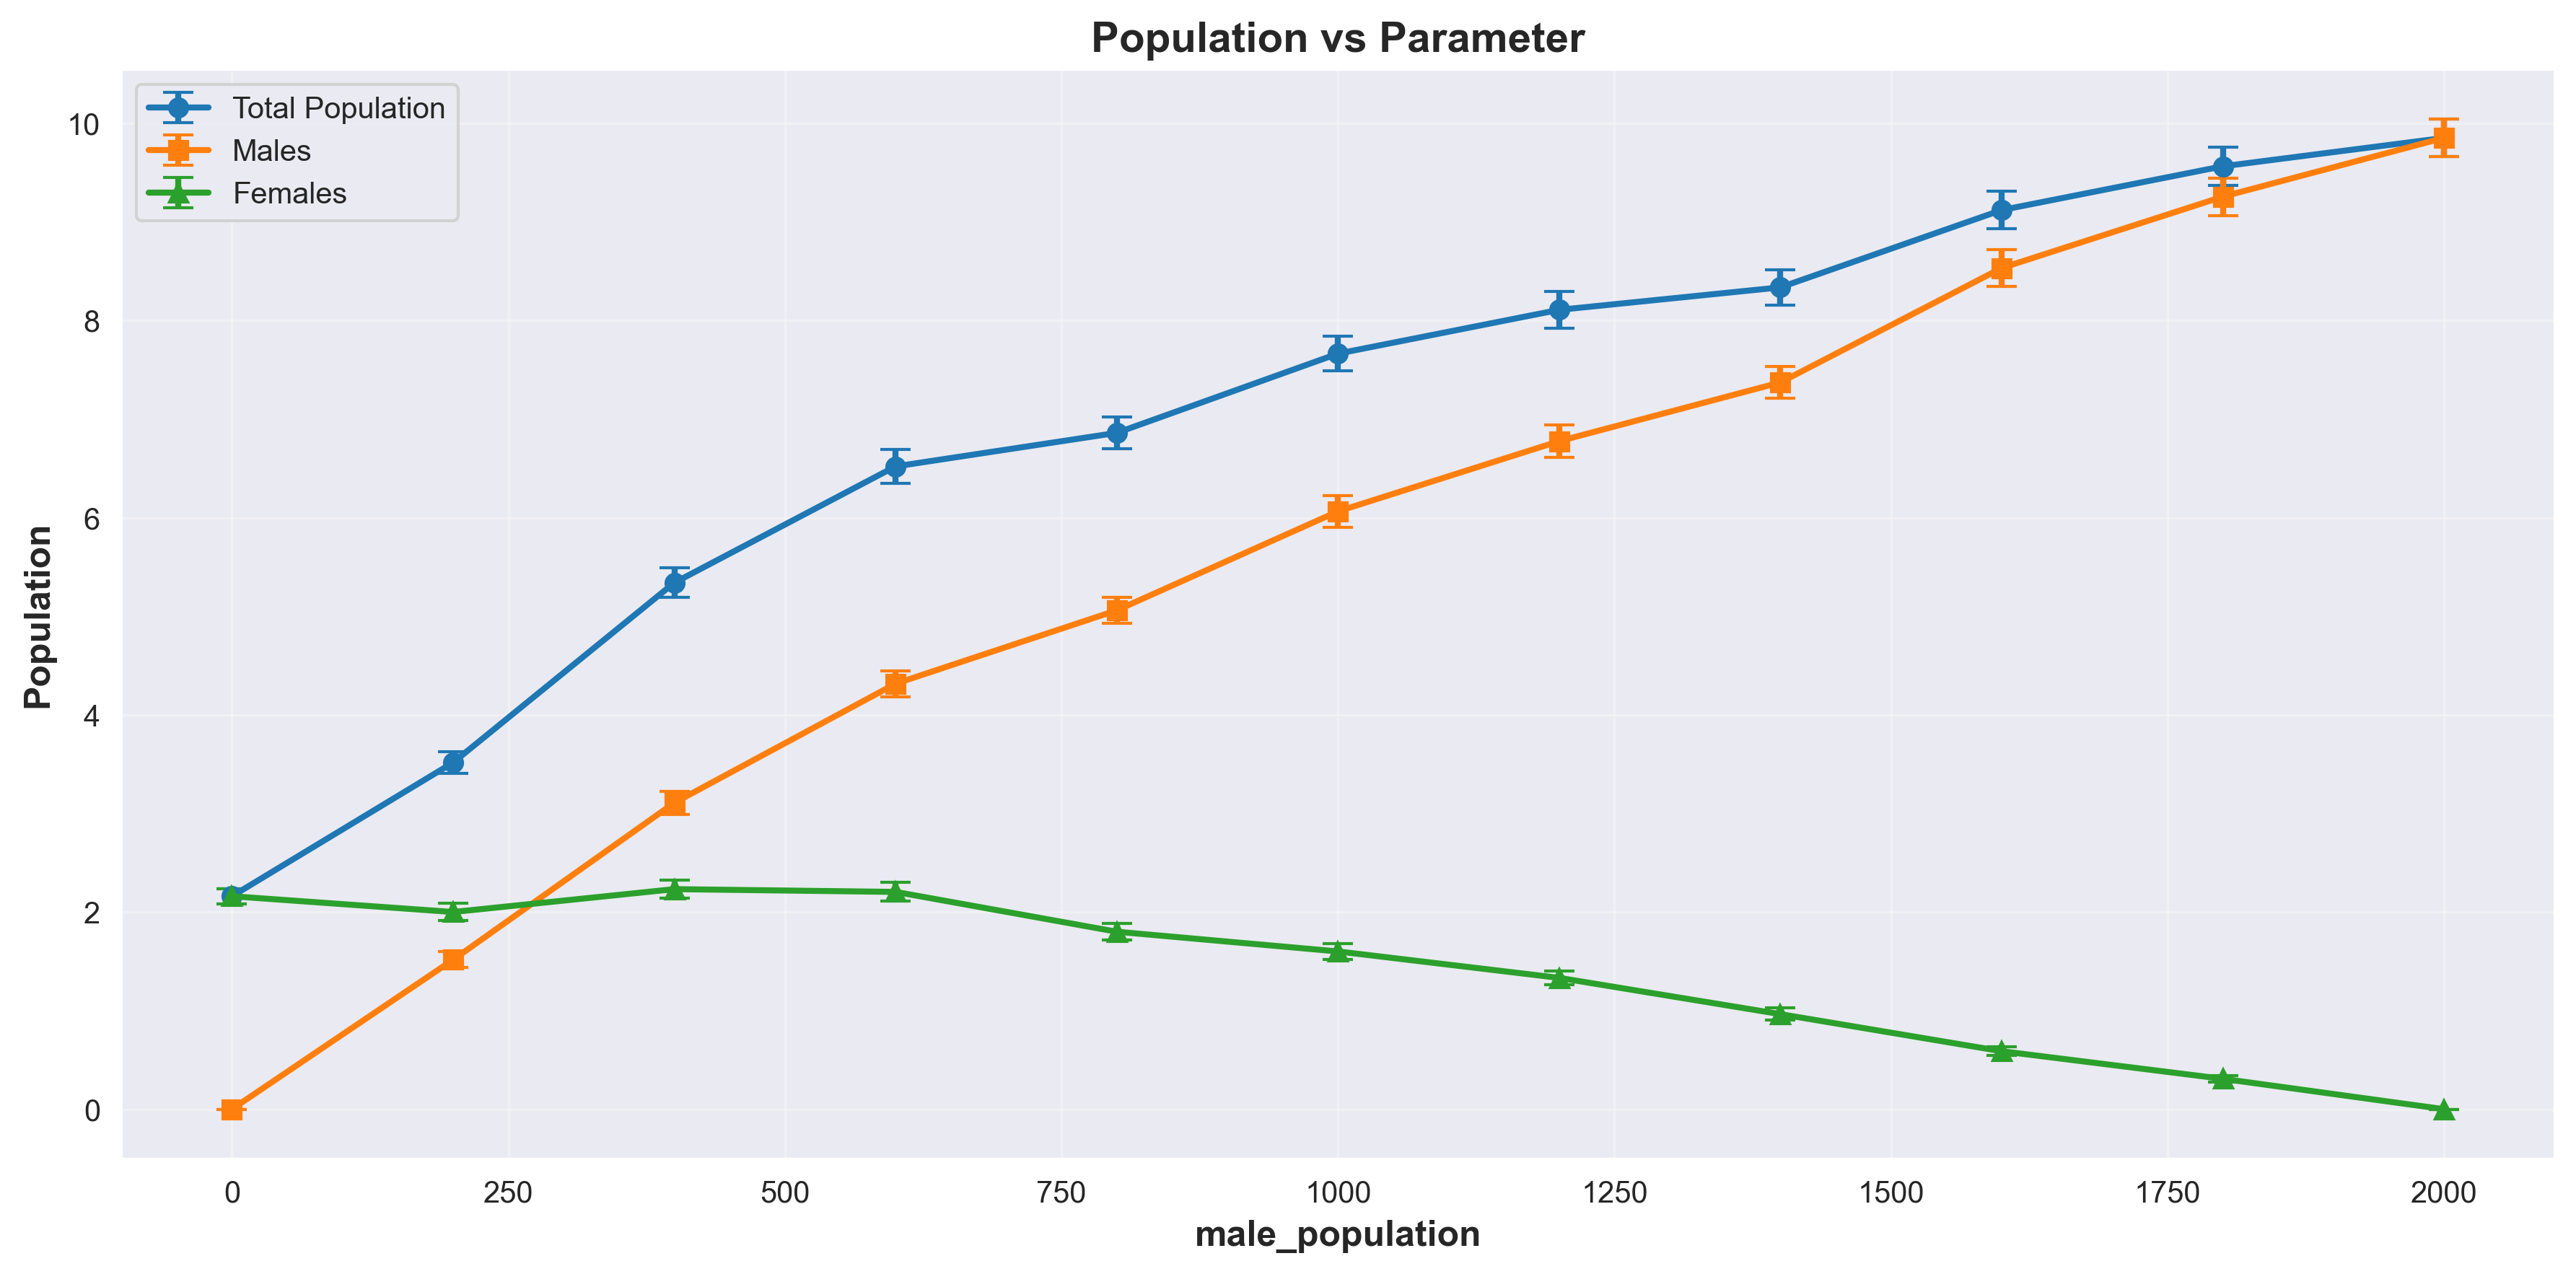
\includegraphics[width=0.9\textwidth]{param_population_male.png}
    \caption{Población final en función de la proporción inicial de hombres. Se muestran la media y bandas de error estándar (media $\pm$ SE) para 250 réplicas por valor de parámetro.}
    \label{fig:param_pop}
\end{figure}

\subsubsection{Dinámicas de Sexos}

La razón de sexos (M/F) exhibe un comportamiento altamente sensible a la condición inicial, con implicaciones profundas para la dinámica reproductiva. Como se observa en la Figura \ref{fig:param_sratio} y como se comentaba anteriormente, la distribución ideal de $0.5 - 2.0$ se encuentra entre los valores de población inicial masculina entre $200$ y $600$, sugiriendo que explorar la evolución a largo plazo de una población con estos valores iniciales puede resultar interesante.

\begin{figure}[h]
    \centering
    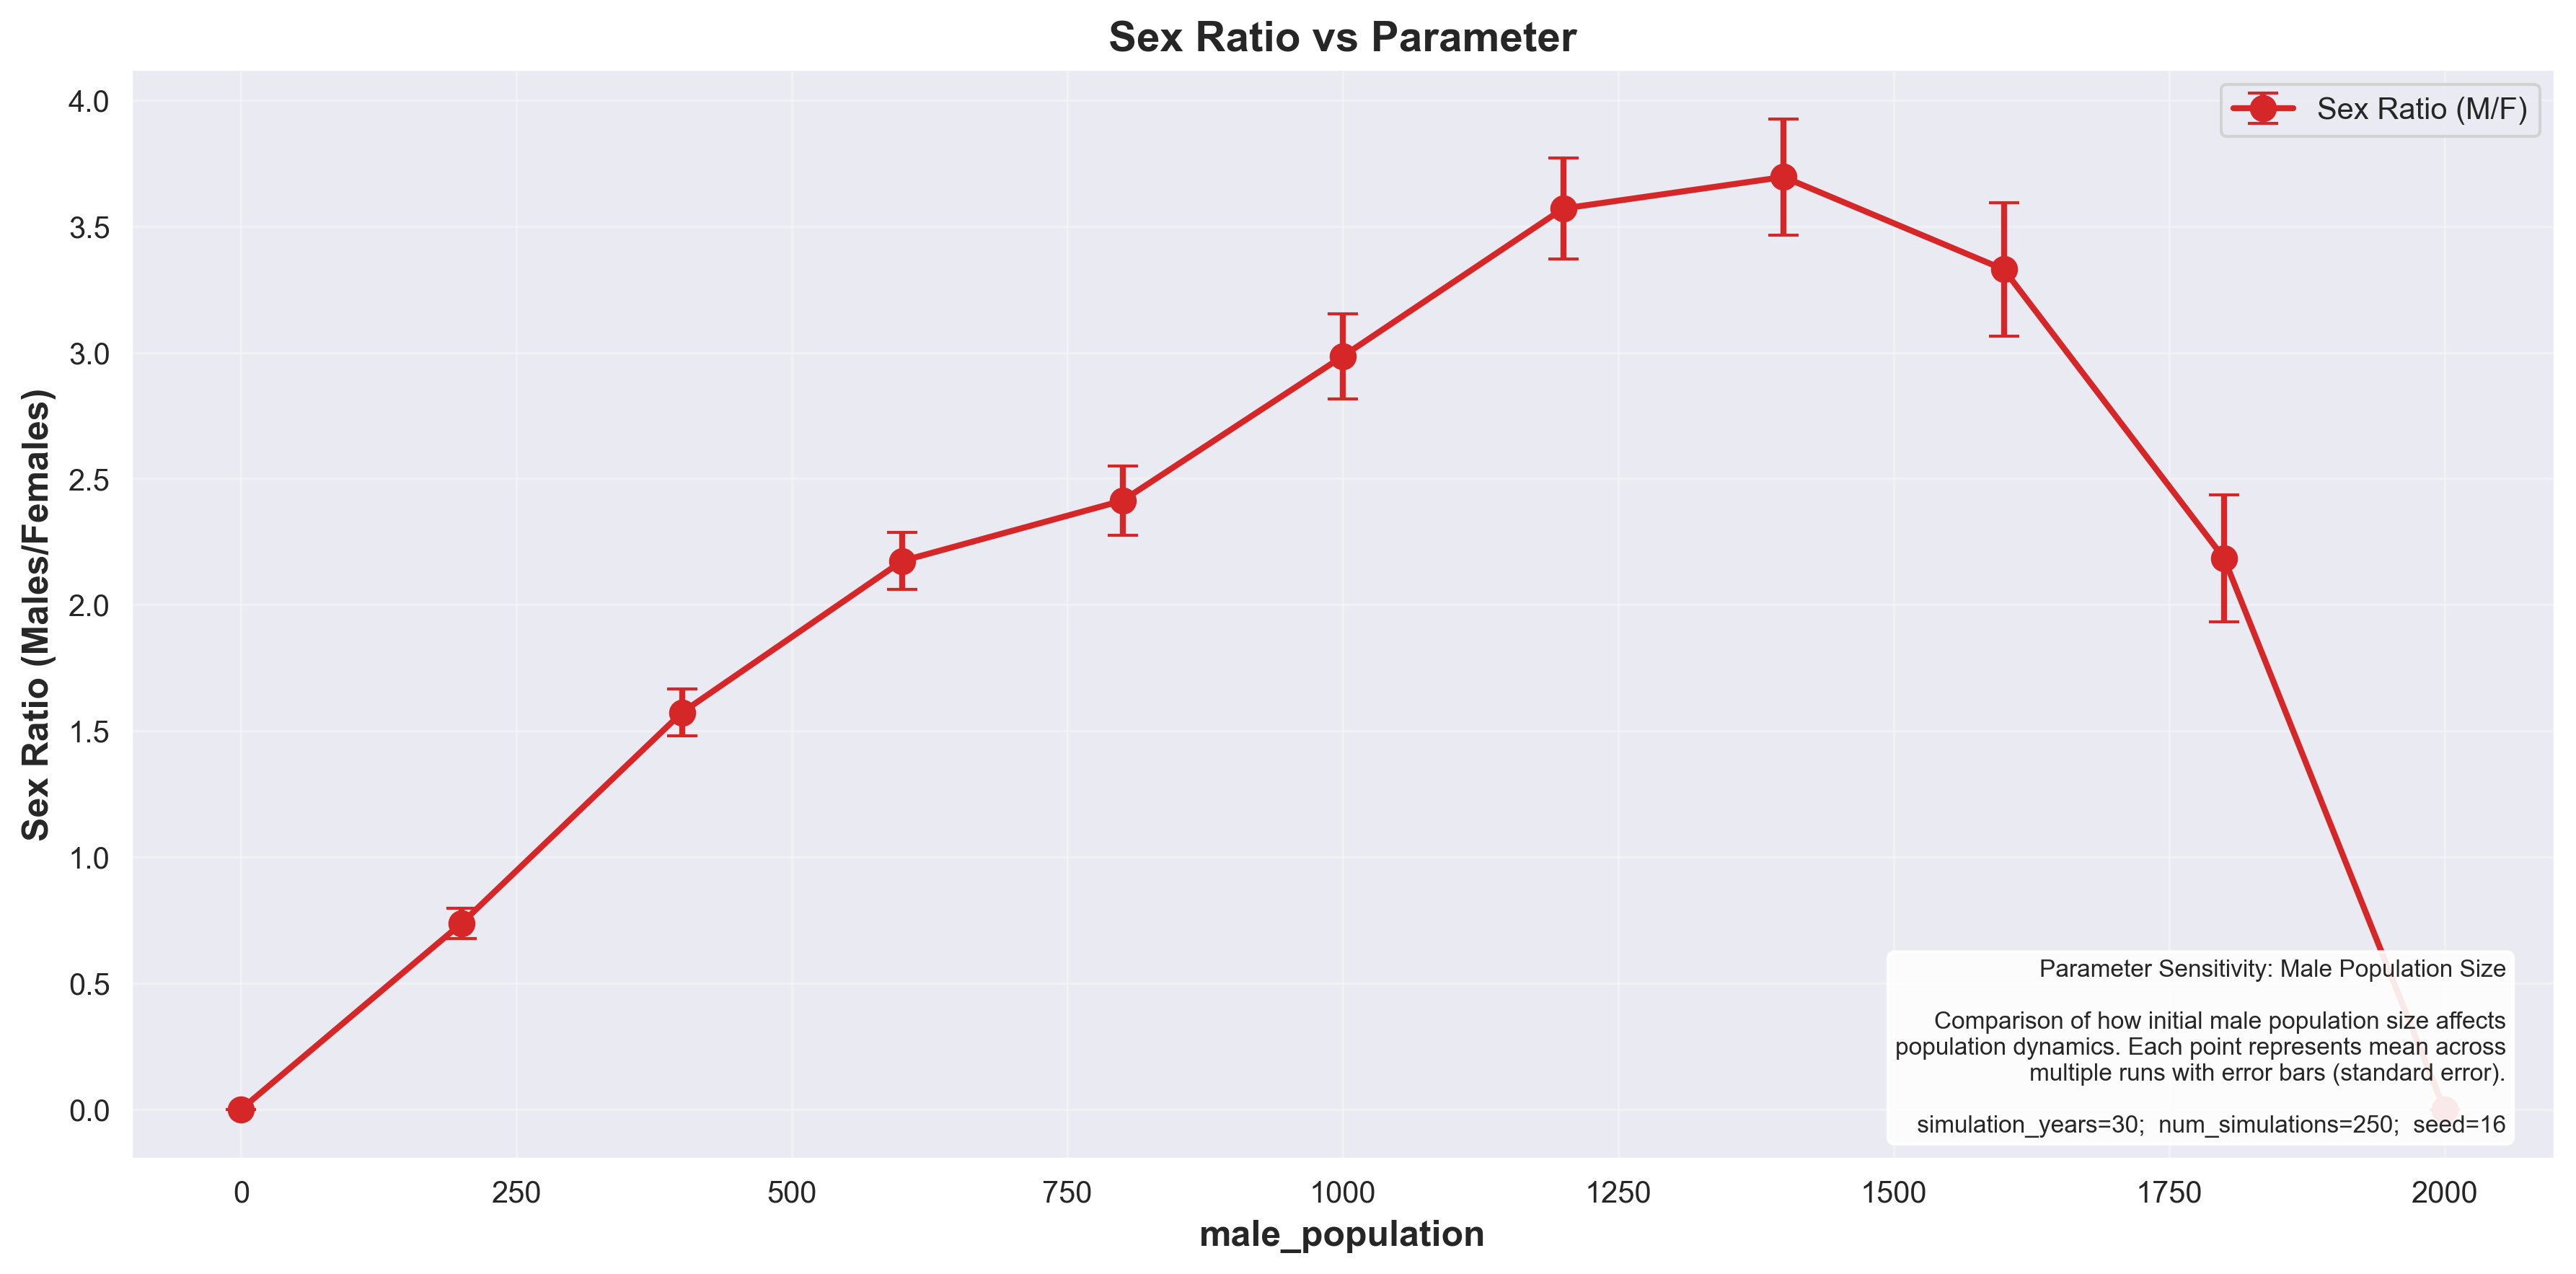
\includegraphics[width=0.9\textwidth]{param_sratio_male.png}
    \caption{Razón de sexos (M/F) en función de la población inicial masculina. Las bandas de error muestran el error estándar a través de las 250 réplicas.}
    \label{fig:param_sratio}
\end{figure}

\subsubsection{Edad Promedio}

La edad promedio final mostrada en la Figura \ref{fig:param_age} refleja que los extremos de distribución de sexos (0 y 2000 hombres iniciales) producen poblaciones significativamente más envejecidas, con edades promedio superiores a 44 años, lo cual tiene sentido debido a que no se producen nacimientos prácticamente y la población tiende a envejecer constantemente. Un efecto similar puede observarse para los valores más altos de población inicial masculina, donde la edad y la cantidad de supervivientes está ampliamente influenciada por la mayor predisposición a la supervivencia de los hombres y la baja tasa de natalidad esperada al haber menor cantidad de mujeres presentes en la población. Nuevamente, los mejores valores son observados para valores iniciales de población masculina entre $200$ y $800$, dado que una población más joven indica una mayor probabilidad de regenerarse en el tiempo debido a la mayor probabilidad de reproducción de las personas en edades jóvenes.

\begin{figure}[h]
    \centering
    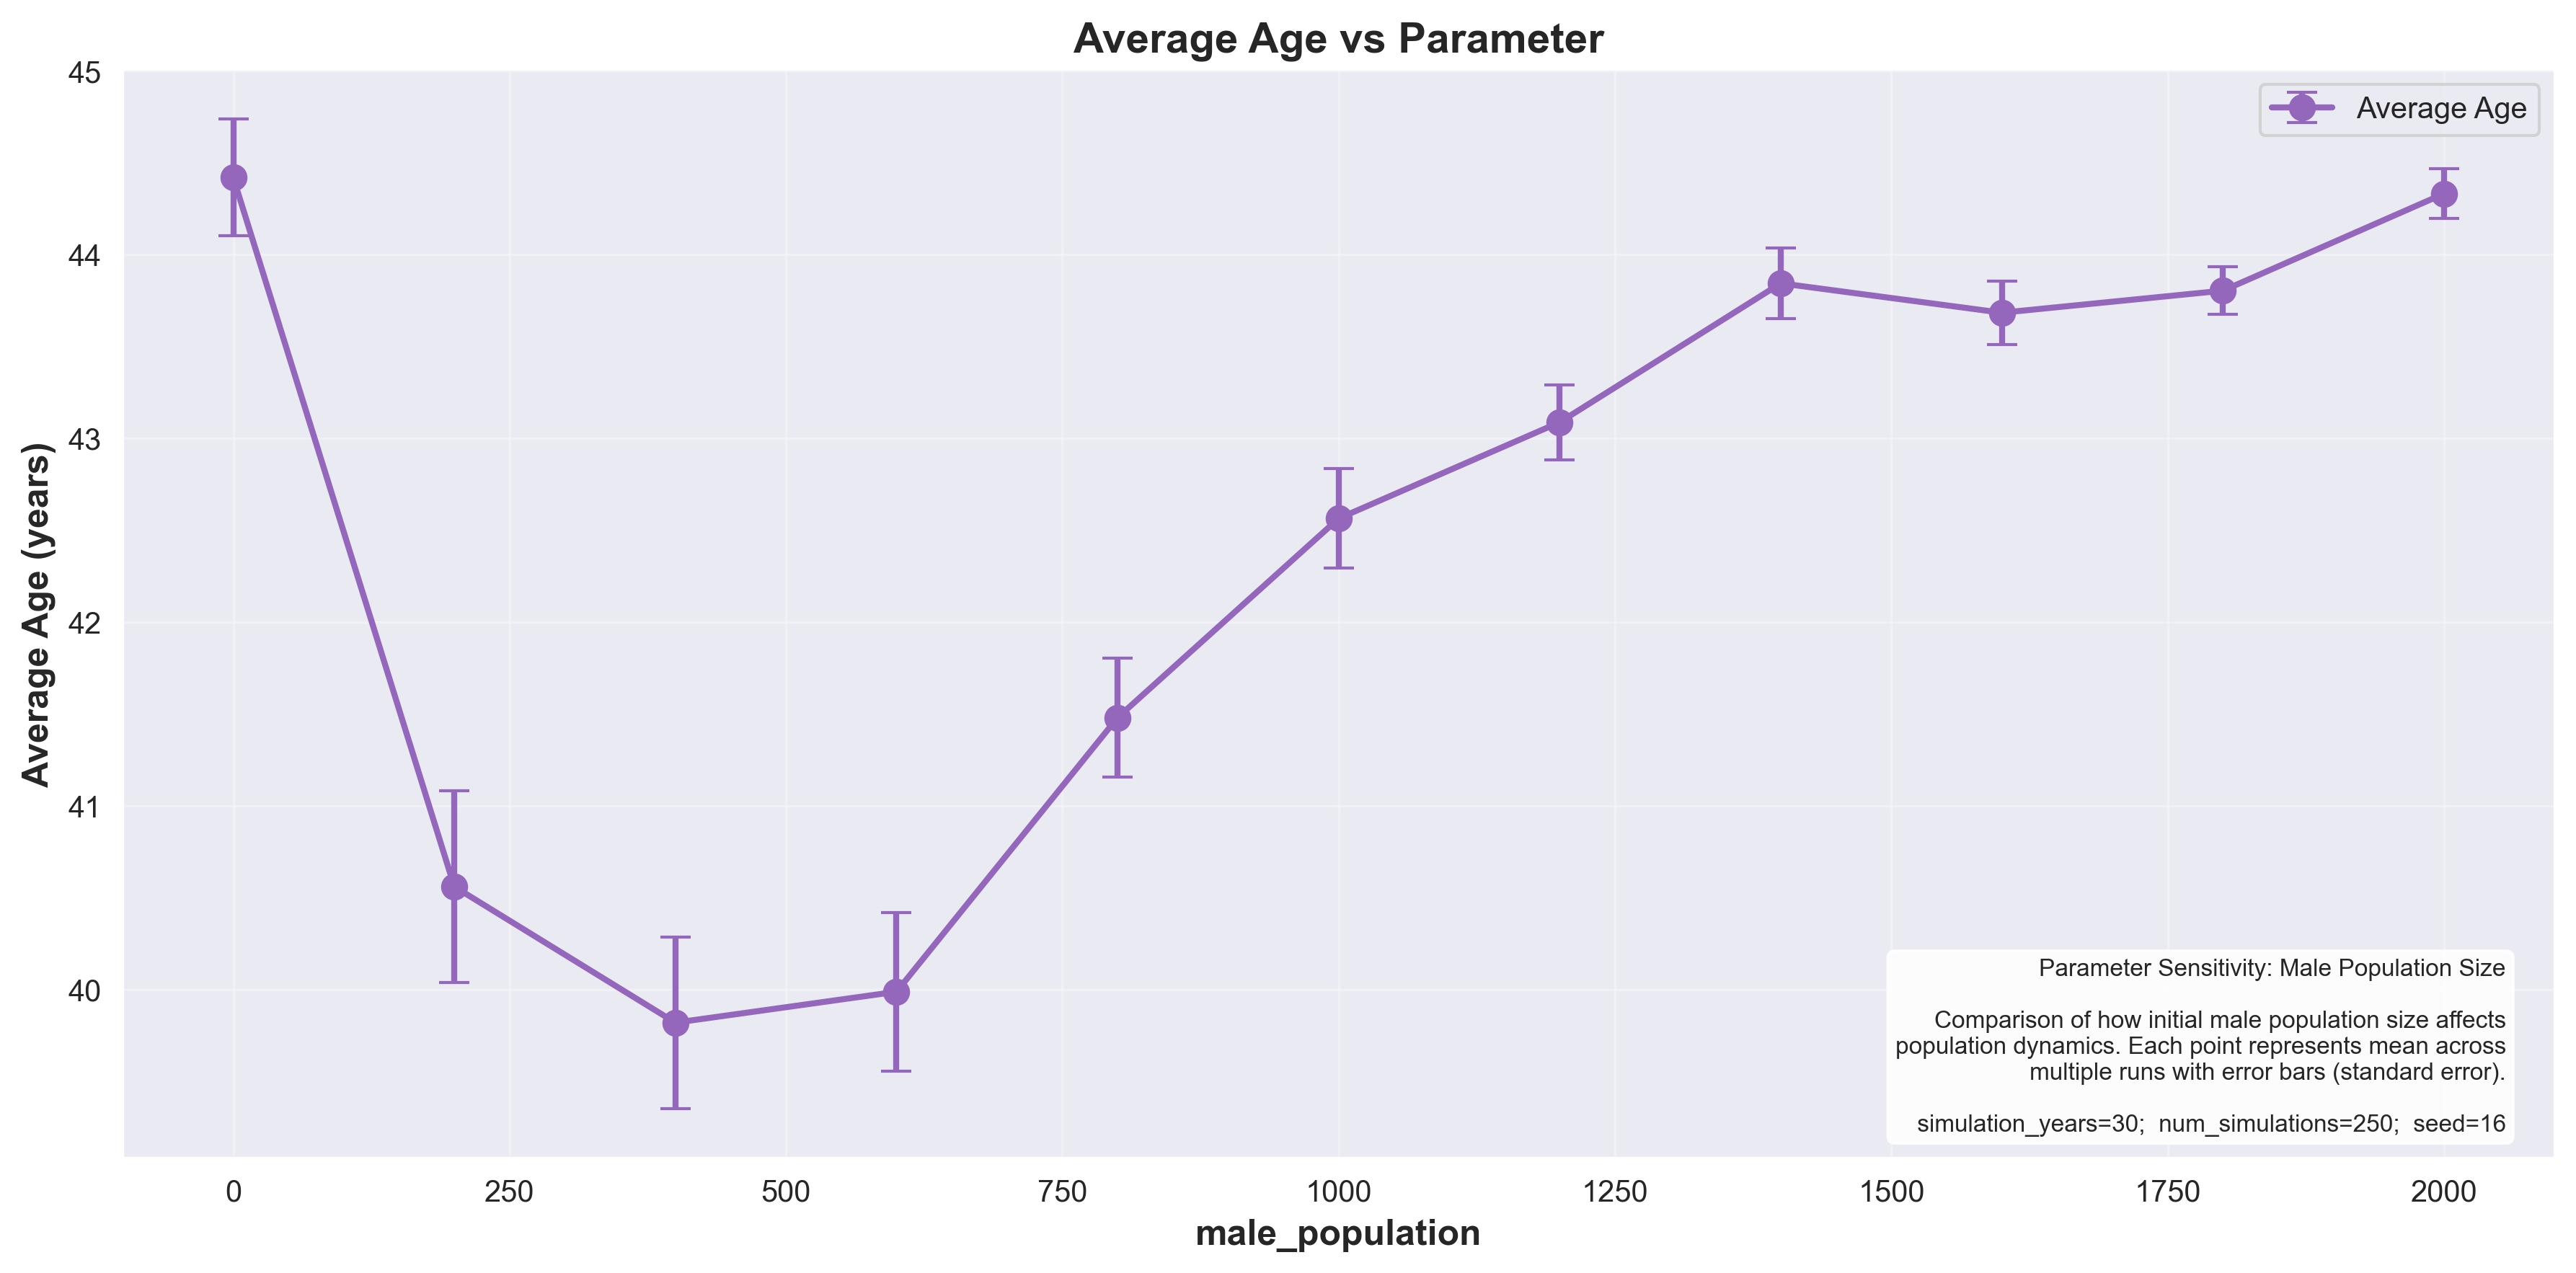
\includegraphics[width=0.9\textwidth]{param_age_male.png}
    \caption{Edad promedio final en función de la población inicial masculina. Se representan la media y el error estándar para las 250 réplicas. Poblaciones con distribuciones de sexos más balanceadas resultan en estructuras etarias ligeramente más jóvenes, reflejando una tasa de reemplazo generacional superior.}
    \label{fig:param_age}
\end{figure}

El análisis de sensibilidad paramétrica demuestra que la viabilidad poblacional depende de un delicado equilibrio entre la proporción de sexos y la capacidad reproductiva emergente. Las simulaciones indican que poblaciones con aproximadamente 60-70\% de hombres iniciales (correspondiente a 1200-1400 individuos de una población de 2000) maximizan las perspectivas de supervivencia a corto plazo en el horizonte de 30 años, mientras poblaciones con aproximadamente 10-40\% de hombres iniciales (correspondiente a 200-800 individuos de una población de 2000) sugieren mayor supervivencia a largo plazo. Este resultado tiene implicaciones para la comprensión de poblaciones reales sometidas a desequilibrios severos de sexos, ya sea por fuertes mortalidades selectivas o migraciones diferenciadas.

\section{Experimento 3: Evolución simple con distribución de sexos fija}

\subsection{Objetivo}

Estudiar cómo evoluciona la población en el tiempo bajo los parámetros demográficos especificados y con una distribución de sexos fija que beneficia la cantidad de mujeres.

\subsection{Parámetros Iniciales}

\begin{itemize}
	\item Población inicial: \texttt{2000}
	\item Población inicial masculina: \texttt{500}
	\item Duración de simulación: \texttt{100}
	\item Número de réplicas por experimento: \texttt{500}
	\item Edad mínima de fertilidad: \texttt{12}
	\item Edad máxima de fertilidad: \texttt{70}
	\item Edad mínima de emparejamiento: \texttt{12}
	\item Edad máxima: \texttt{125}
	\item Semilla: \texttt{16}
\end{itemize}

A partir de los resultados obtenidos en el experimento anterior \ref{sec:exp2} que sitúan la situación más prometedora a futuro alrededor de una distribución cercana al $25\%$ de hombres iniciales (correspondiente a aproximadamente $500$ individuos de una población de $2000$), se decidió correr nuevamente la simulación a largo plazo con este ratio para comparar la evolución poblacional y evaluar si la proporción de sexos mejorada produce dinámicas más favorables en el horizonte de 100 años.

\subsection{Resultados}

\subsubsection{Dinámica Poblacional}

Contrario a las expectativas iniciales basadas en los hallazgos del Experimento 2, la población con distribución de sexos 500:1500 (M:F) exhibe una tendencia de extinción prácticamente idéntica a la observada en el Experimento 1. Como puede observarse en la Figura \ref{fig:pop_evolution_exp3}, la población declina de manera casi exponencial durante los primeros 40 años y prácticamente llegando a la extinción antes del año 50. La tasa de declinación es extremadamente rápida en los primeros 10 años, donde la población pasa de 2000 a aproximadamente 217 individuos. Este resultado sugiere que la limitación crítica para la viabilidad poblacional no es únicamente la proporción de sexos en términos de cantidad, sino más bien la interacción compleja entre la estructura etaria inicial, las tasas de mortalidad, y la tasa de fertilidad de las mujeres en edad reproductiva. Un ratio de hombres al 25\% aparentemente no proporciona la capacidad reproductiva suficiente para contrarrestar la mortalidad observada en la población.

\begin{figure}[h]
    \centering
    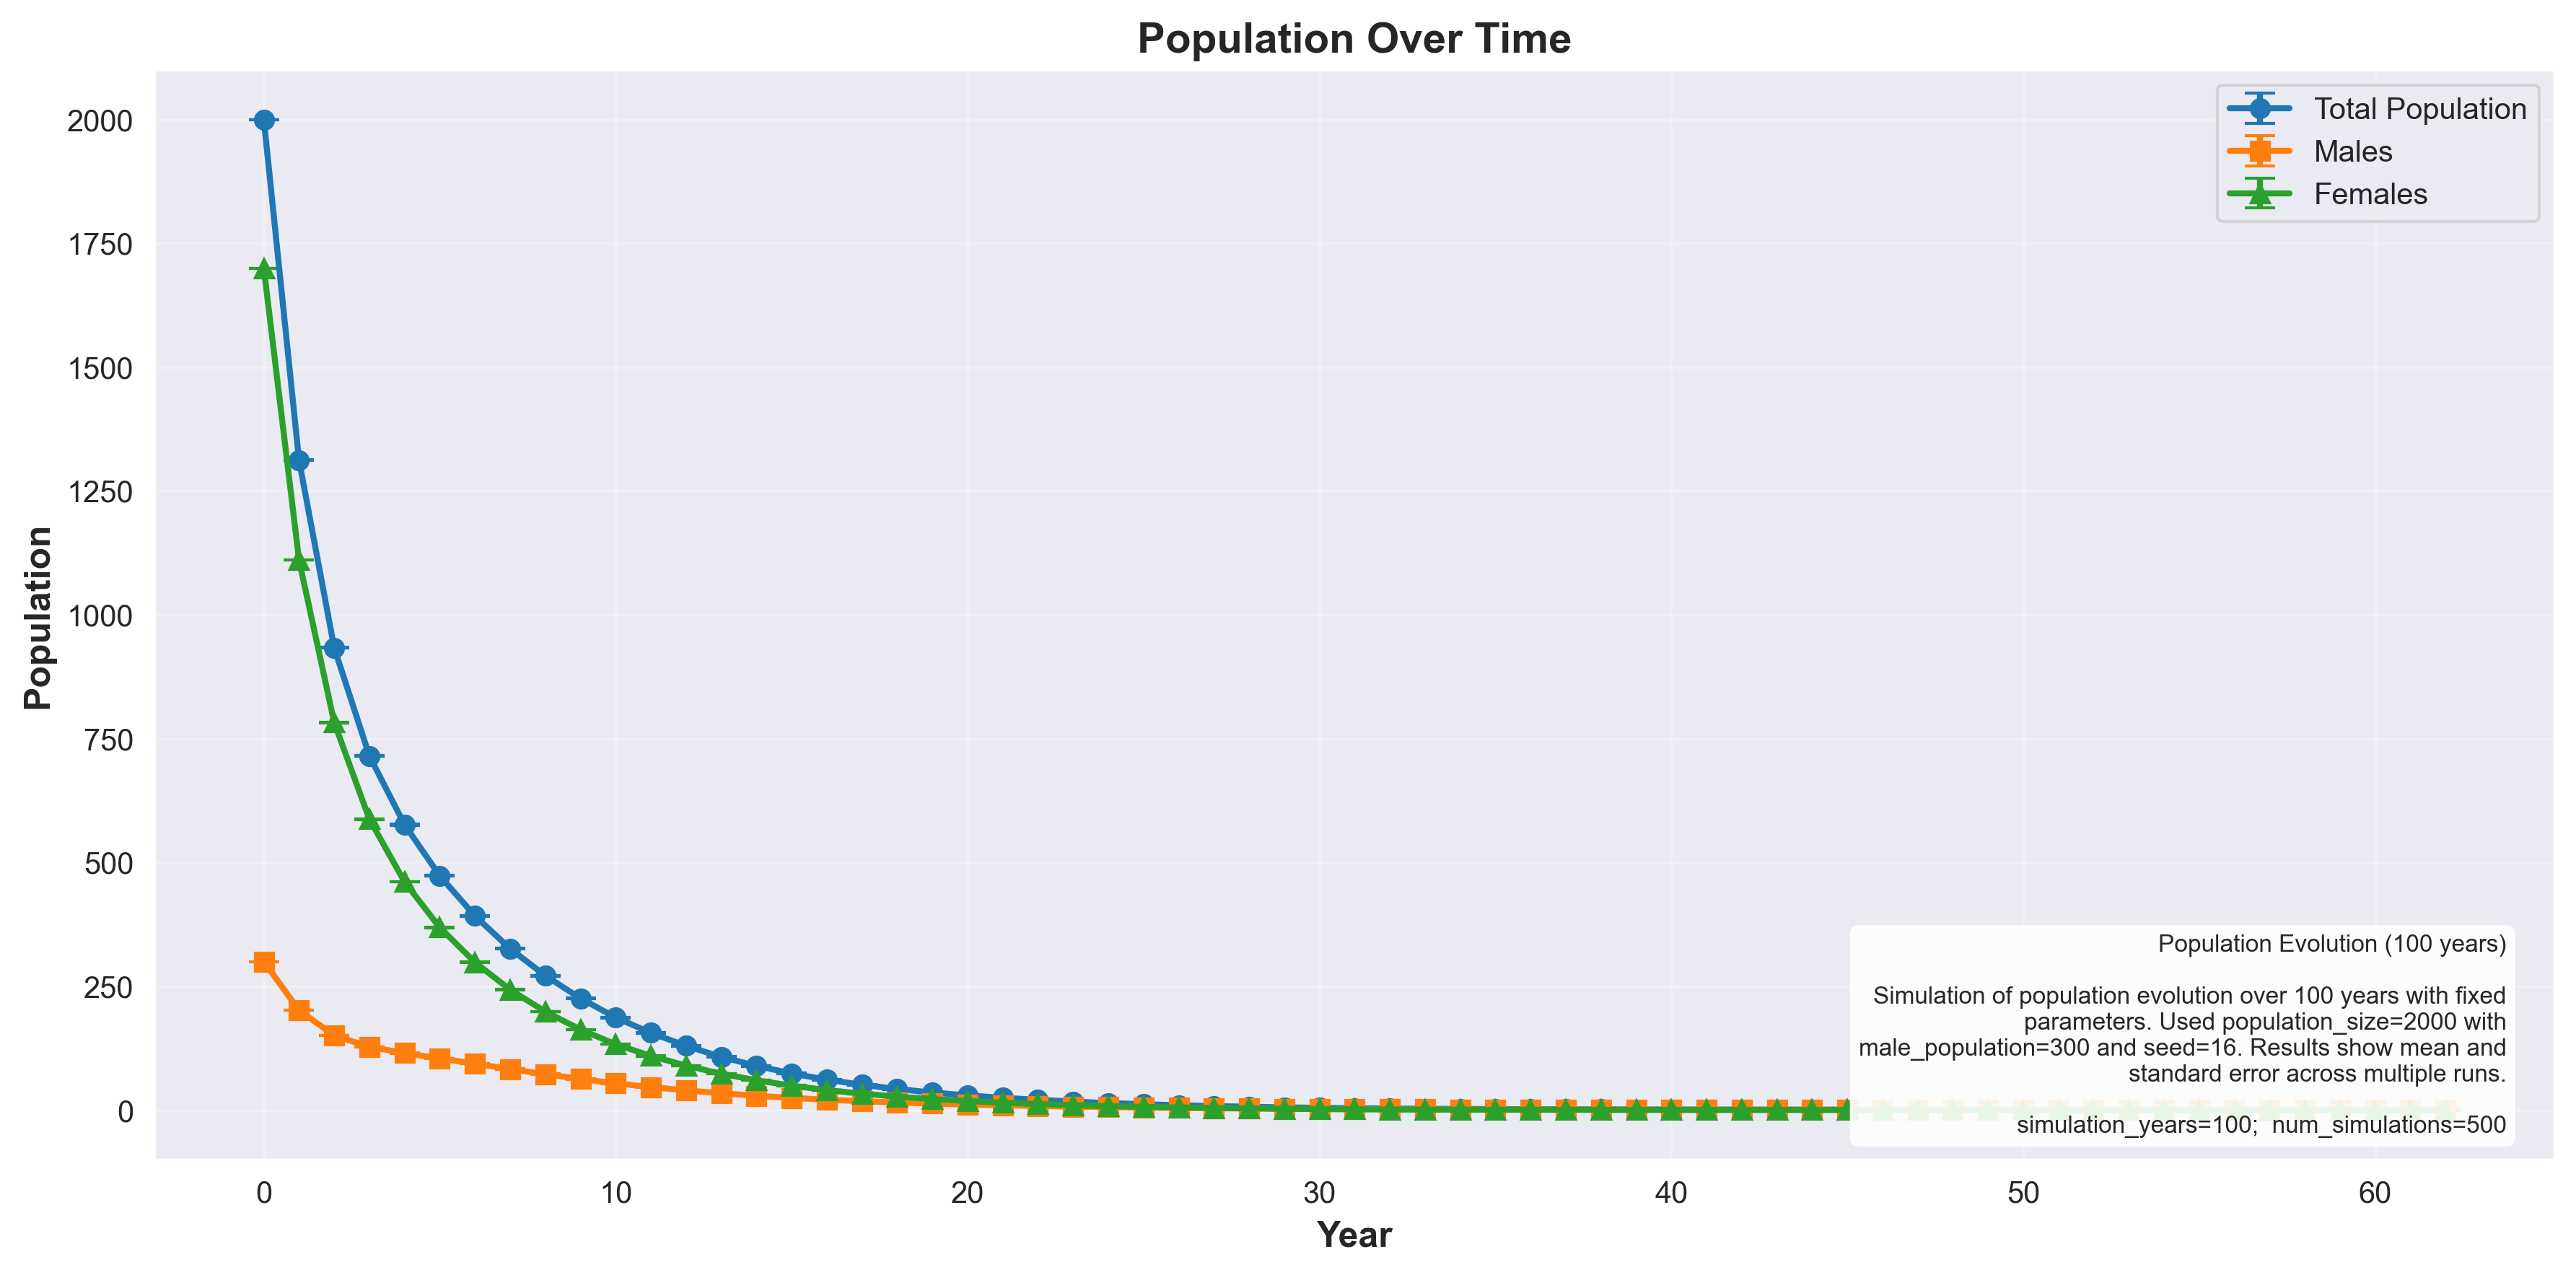
\includegraphics[width=0.9\textwidth]{simple_population_2000_500.png}
    \caption{Evolución de la población por sexo usando 500 hombres y 1500 mujeres iniciales en 100 años de simulación (500 réplicas). Se muestran hombres (naranja), mujeres (verde) y población total (azul) con bandas de error estándar. La tendencia a la extinción es pronunciada y comparable a la vista en la Figura \ref{fig:pop_evolution}.}
    \label{fig:pop_evolution_exp3}
\end{figure}

\subsubsection{Dinámicas de Sexos}

La razón de sexos muestra un comportamiento que refleja selectivamente la supervivencia diferencial por sexo bajo esta configuración inicial. Como se ilustra en la Figura \ref{fig:sex_ratio_exp3}, la razón M/F comienza en $0.33$ (correspondiente a 500 hombres sobre 1500 mujeres) pero aumenta progresivamente durante los primeros 30 años de simulación, alcanzando un valor óptimo cerca del año 20 antes de desbalancearse y caer nuevamente hacia 0 en los años finales. Este patrón sugiere que en las primeras décadas, cuando aún hay individuos vivos, los hombres son relativamente favorecidos en supervivencia, lo que causa una convergencia de la razón de sexos hacia $2.0$. Sin embargo, la caída final de la razón hacia $0$ refleja la extinción prácticamente simultánea de ambos sexos.

\begin{figure}[h]
    \centering
    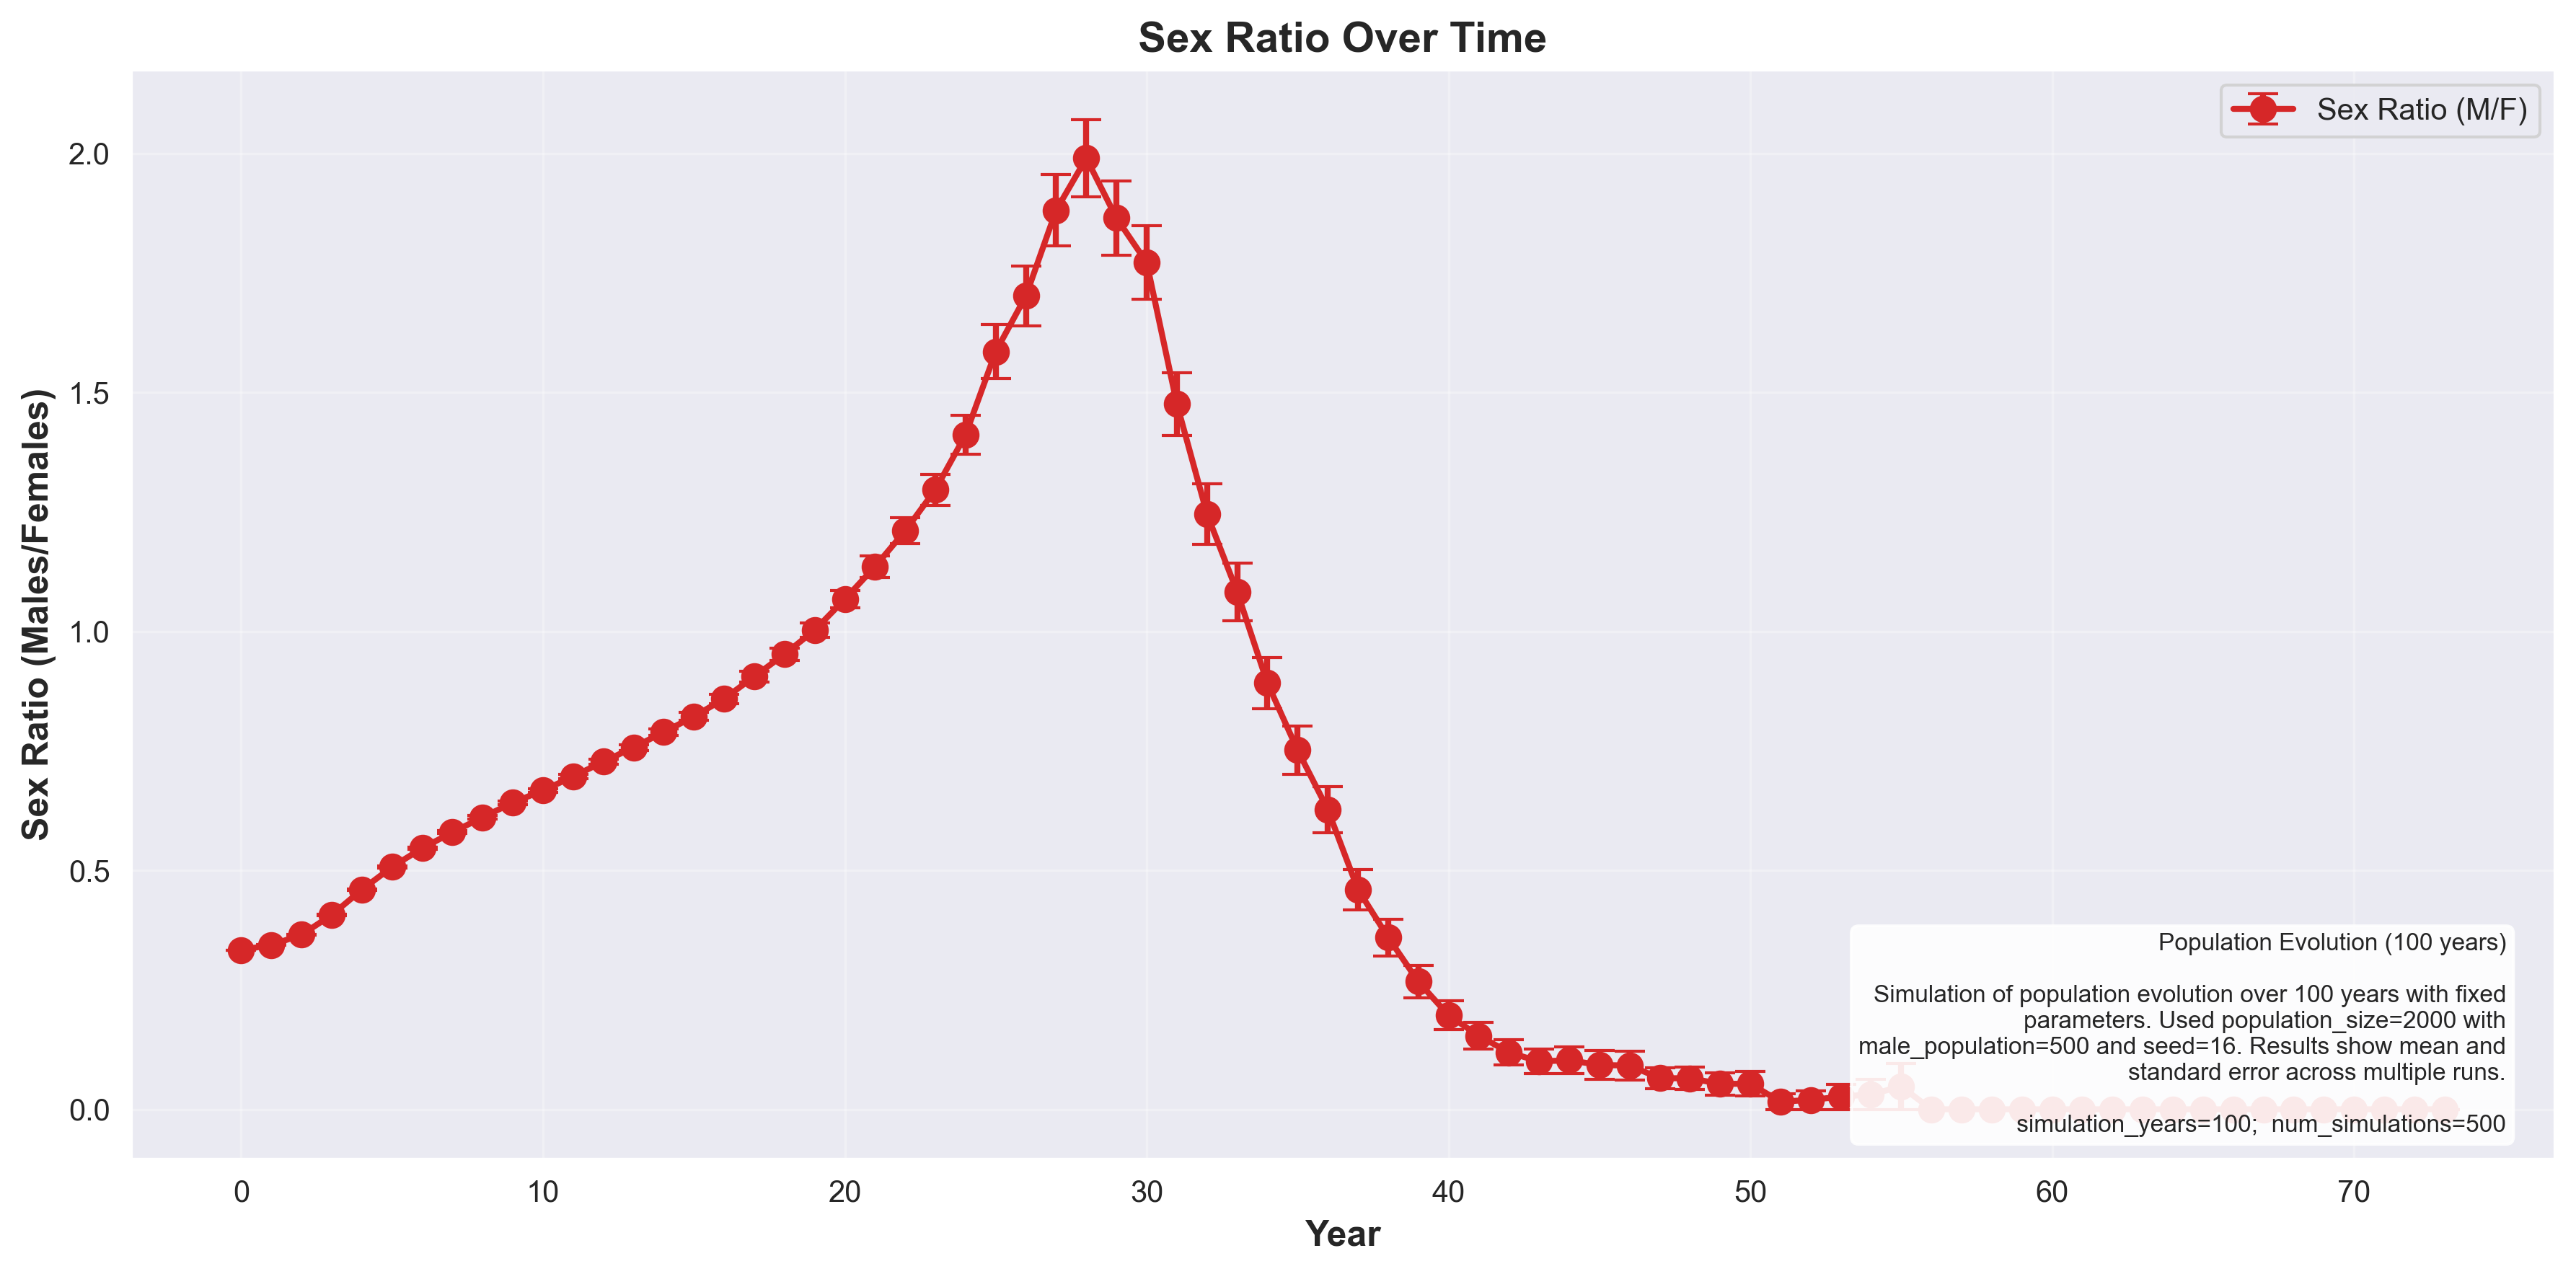
\includegraphics[width=0.9\textwidth]{simple_sratio_2000_500.png}
    \caption{Razón de sexos (M/F) en función del tiempo de las simulaciones. Se observa un aumento inicial seguido de estabilización y posterior declinación hacia cero a medida que la población se extingue.}
    \label{fig:sex_ratio_exp3}
\end{figure}

\subsubsection{Edad Promedio}

La edad promedio presentada en la Figura \ref{fig:avg_age_exp3} sigue el patrón esperado de una población en extinción. Comienza alrededor de 51 años (reflejando la distribución uniforme inicial de edades en [0, 100]), desciende rápidamente a aproximadamente 28-30 años entre los años 5 y 15, donde se estabiliza por un período. Durante esta estabilización, la población mantiene una estructura etaria relativamente joven debido a la presencia de individuos en rangos reproductivos. Sin embargo, a partir del año 25-30, conforme la población envejece y disminuye drásticamente, la edad promedio comienza a aumentar nuevamente, alcanzando valores superiores a 45 años por el año 55. Este repunte tardío refleja el envejecimiento de los últimos supervivientes sin reemplazo generacional, dado que la baja tasa de natalidad no compensa las muertes.

\begin{figure}[h]
    \centering
    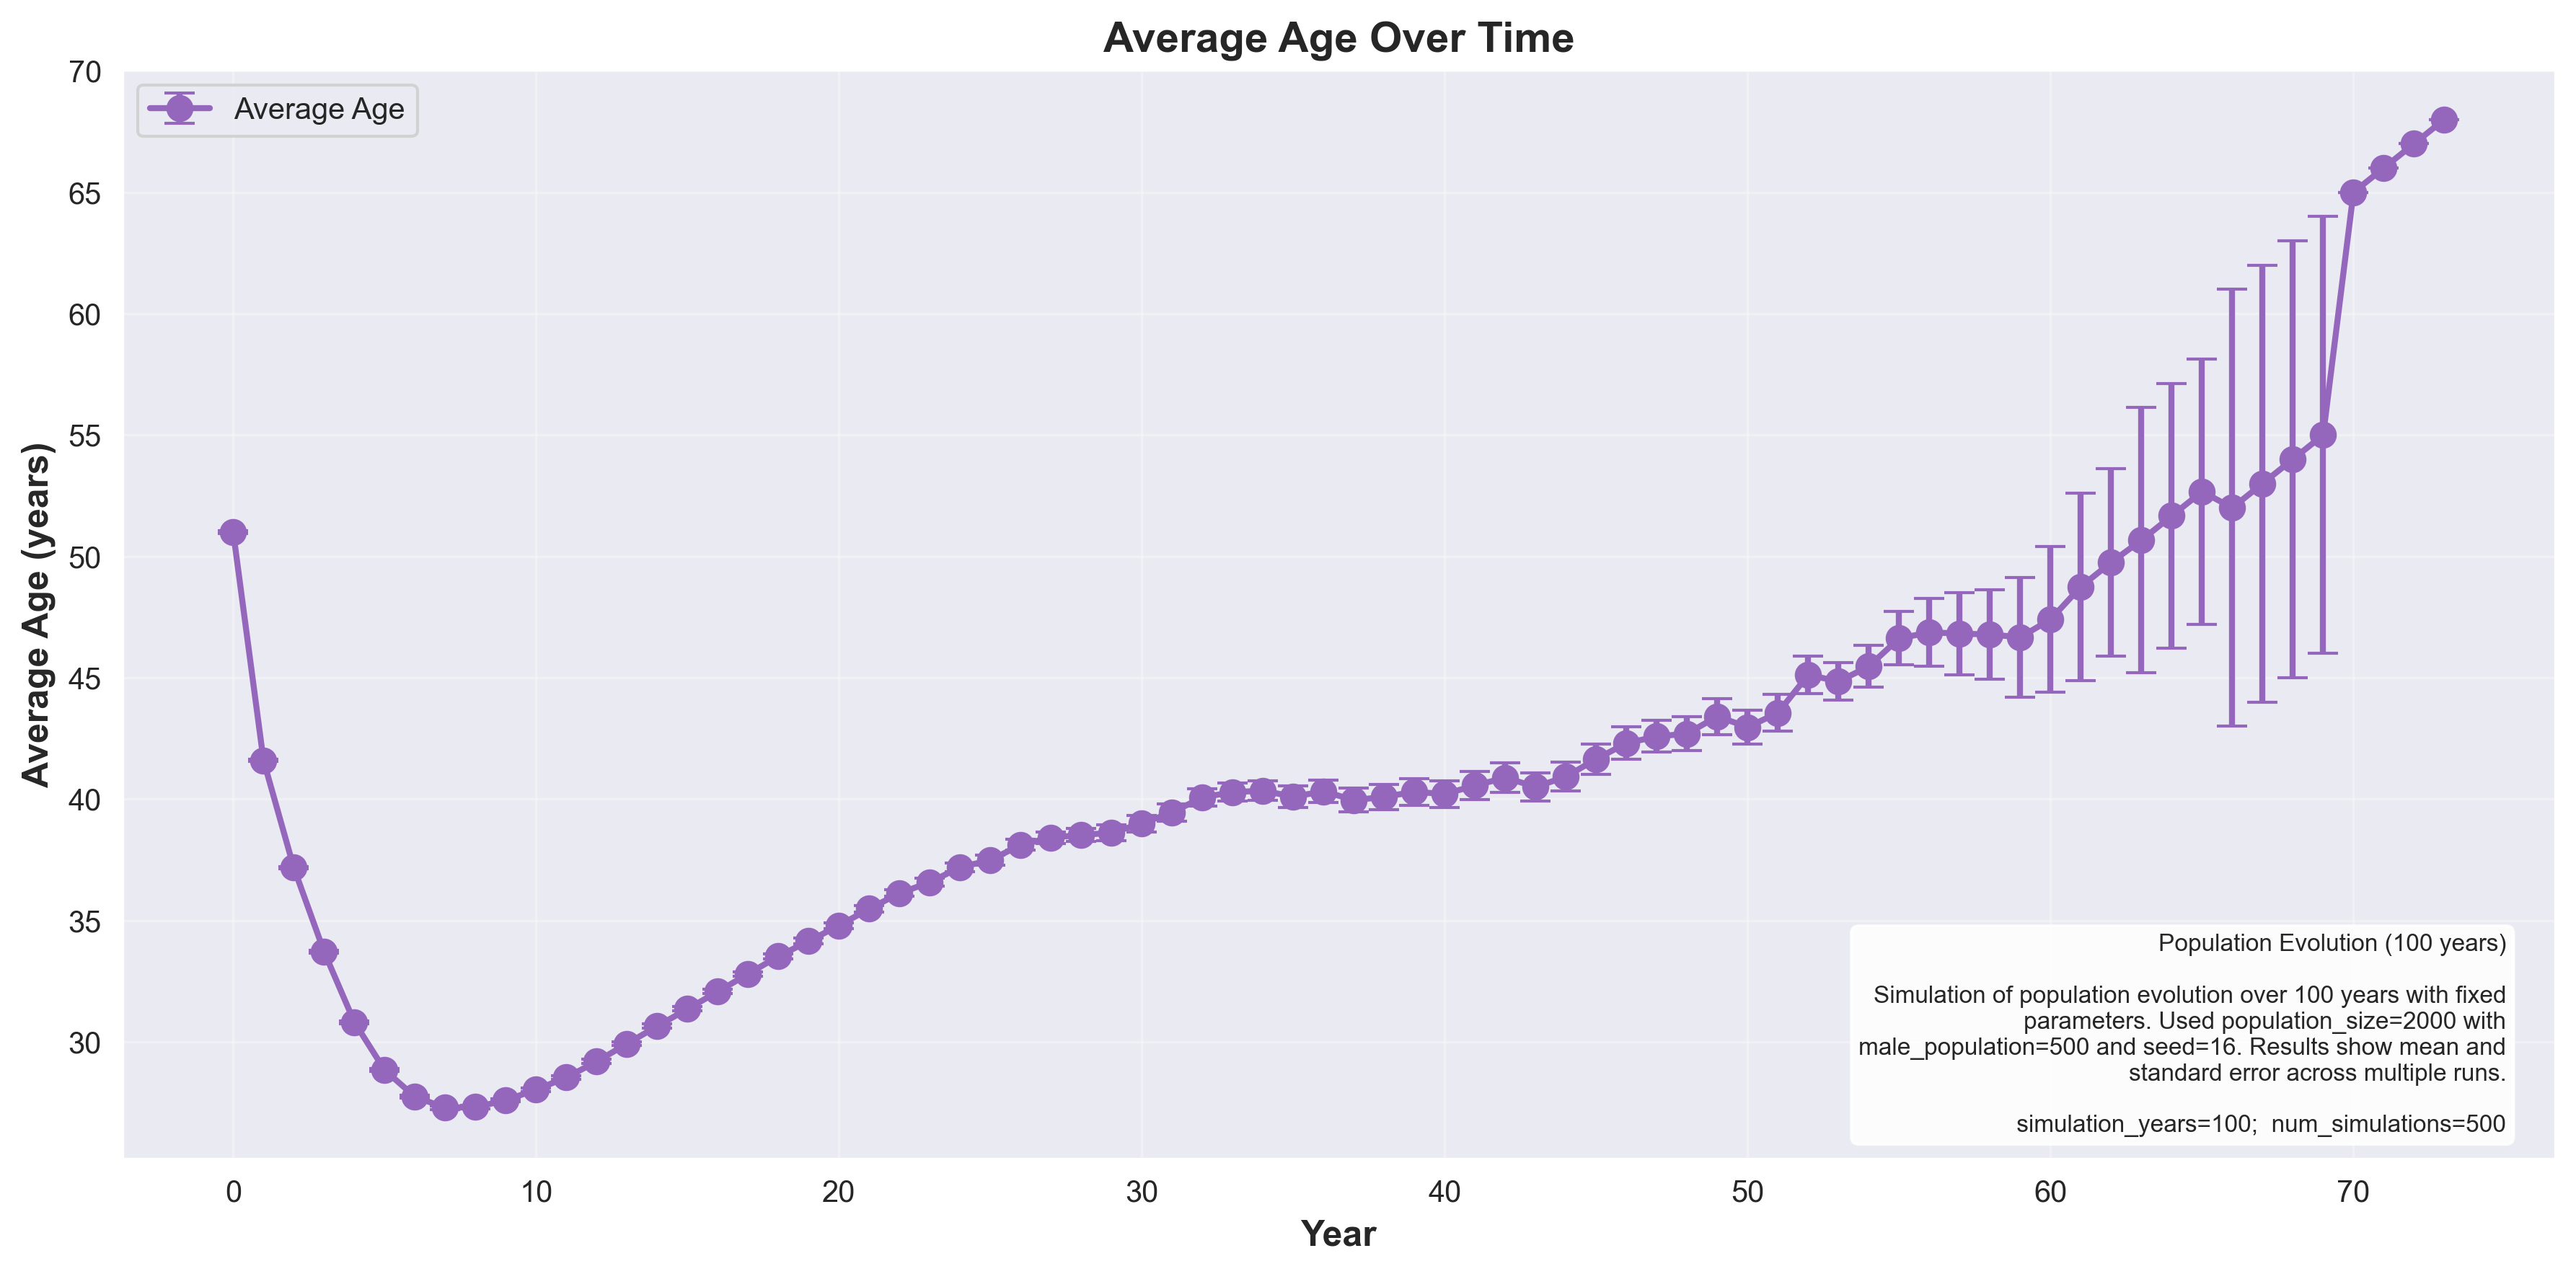
\includegraphics[width=0.9\textwidth]{simple_age_2000_500.png}
    \caption{Edad promedio de la población en función del tiempo. Se evidencia el descenso inicial seguido de estabilización y posterior envejecimiento conforme la población se aproxima a la extinción.}
    \label{fig:avg_age_exp3}
\end{figure}

Queda demostrado que ajustar la proporción inicial de sexos hacia una mayor representación femenina (500 hombres: 1500 mujeres) no logra mitigar la problemática fundamental identificada en los experimentos previos. La extinción poblacional persiste con dinámicas prácticamente equivalentes a las de \ref{sec:exp1}, sugiriendo que los parámetros demográficos fundamentales del modelo (especialmente las tasas de fertilidad, mortalidad, y formación de parejas) pueden requerir una revisión más profunda para permitir una dinámica poblacional estable o al menos de larga duración.



% ============================================================================
% CAPÍTULO 5: CONCLUSIONES
% ============================================================================
\chapter{Conclusiones}

\section{Resumen de Hallazgos}

A través de tres experimentos de simulación demográfica se ha investigado la dinámica poblacional bajo distintos regímenes de parámetros iniciales. El Experimento 1 reveló una tendencia pronunciada a la extinción poblacional en 500 réplicas independientes de 100 años de simulación, con la población alcanzando valores próximos a cero antes del año 70. Esta extinción fue acompañada por una dinámica de sexos en la cual los hombres mostraron supervivencia relativa superior a las mujeres en los primeros años, según se evidenció en la razón de sexos. La edad promedio exhibió un descenso inicial (años 0-10) reflejando la eliminación de individuos envejecidos de la cohorte inicial, seguida de un aumento progresivo indicativo del envejecimiento sin reemplazo generacional.

El Experimento 2 de análisis de sensibilidad paramétrica demostró que la proporción inicial de hombres es un factor de importancia en la dinámica poblacional a corto plazo (30 años). Se identificó que proporciones pequeñas de hombres iniciales (aproximadamente 30-70\%) resultaban en poblaciones finales de mayor tamaño comparado con los extremos (0\% o 100\% de hombres). Específicamente, se observó un máximo de viabilidad poblacional alrededor de 200-800 hombres iniciales de una población de 2000. Sin embargo, incluso bajo estas condiciones favorables, la población final era de menos de 10 individuos tras 30 años, indicando que la mejora en la proporción de sexos solo retarda moderadamente la extinción.

El Experimento 3 confirmó que el ajuste de la proporción de sexos hacia una mayor representación femenina (25\% de hombres iniciales) no logra alterar significativamente las dinámicas de extinción. A pesar de esta reconfiguración, la población exhibió una declinación exponencial comparable a la del Experimento 1, llegando a menos de 150 individuos al año 30 y aproximándose a la extinción antes del año 50. Esto sugiere que la problemática fundamental no radica exclusivamente en la proporción de sexos, sino en la dinámica subyacente de tasas de mortalidad y natalidad del modelo.

\section{Limitaciones del Modelo}

A lo largo del análisis se identificaron varias limitaciones significativas en la estructura demográfica del modelo de simulación. La primera y más evidente es el desequilibrio entre las tasas de mortalidad y natalidad. Las tablas de probabilidad de mortalidad, tal como se describen en el proyecto, producen tasas de defunción que superan sistemáticamente a las tasas de natalidad, impidiendo que la población pueda mantenerse o crecer bajo ninguna configuración paramétrica probada. Esto resulta particularmente problemático considerando que se inicializa la población con edades distribuidas uniformemente en $[0, 100]$, lo cual deja aproximadamente la mitad de la población fuera de los rangos reproductivos, ampliando aún más la brecha entre defunciones y nacimientos.

Una segunda limitación es la capacidad reproductiva restringida del modelo. La tasa de fertilidad, que depende de disponibilidad de parejas fértiles, salud de la madre durante la gestación, y otras condiciones estocásticas, resultó ser insuficiente en todas las configuraciones simuladas para mantener el reemplazo poblacional. La dinámica de formación de parejas, además, introduce restricciones adicionales que reducen la probabilidad efectiva de reproducción.

Una tercera limitación concierne a la representación de edades iniciales. La asignación uniforme de edades en $[0, 100]$ años, aunque computacionalmente simple, no refleja la estructura etaria típica de poblaciones reales, las cuales generalmente exhiben patrones de pirámide poblacional con concentración en edades más jóvenes. Esta desviación podría contribuir al sesgo hacia la extinción observado.

Finalmente, el modelo incorpora eventos adicionales no especificados en la orden (específicamente el evento \texttt{YearEndEvent}) para distribuir eventos como muertes y separaciones mes a mes. Si bien esta aproximación añade realismo, también introduce complejidad que podría estar interactuando de manera no prevista con los parámetros de probabilidad originales, exacerbando potencialmente el desequilibrio demográfico.

% ============================================================================
% BIBLIOGRAFÍA
% ============================================================================
\begin{thebibliography}{99}

\bibitem{garcia2006}
García Garrido, L., Martí Orosa, L., \& Pérez Sánchez, L. (2006).
\emph{Temas de Simulación}.
Facultad de Matemática y Computación, Universidad de la Habana.

\end{thebibliography}

% ============================================================================
% APÉNDICE: ENLACE AL REPOSITORIO
% ============================================================================
\appendix

\chapter{Información del Proyecto}

\section{Repositorio GitHub}

El código fuente del proyecto se encuentra disponible en:

\begin{center}
    \url{https://github.com/sebagonz106/Discrete-Events}
\end{center}

\section{Estructura del Repositorio}

El repositorio contiene:

\begin{itemize}
    \item Código fuente Julia del simulador
    \item Script de Python para visualización
    \item Archivos de configuración
    \item Documentación técnica
    \item Resultados de simulaciones
\end{itemize}

\section{Instrucciones de Uso}

Para reproducir los resultados:

\begin{enumerate}
    \item Clonar el repositorio
    \item Instalar dependencias Julia y Python
    \item Ejecutar \texttt{julia main.jl} para realizar simulaciones
    \item Ejecutar \texttt{python plot.py} para generar visualizaciones (requiere resultados previos)
\end{enumerate}

\end{document}
